\chapter{Girando in tondo: dal cerchio all'orbita di Halley} \label{cap:cerchio}

\section{Low floor...}

\begin{figure}[h]
   \centering
   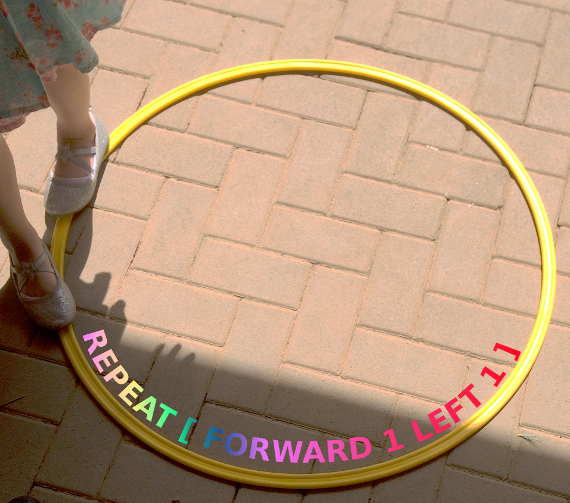
\includegraphics[width=12.0cm]{./images/cerchio/PiccolomanualeLibreLogo5-img1.png}
   \caption{Per le fotografie da cui ho tratto le immagini e per buona parte dei testi in questa sezione sono debitore della maestra Antonella Colombo che ringrazio per avere condiviso le sue preziose esperienze.}
   \label{bambina-gira}
\end{figure}

Percorrendo il caotico dibattito intorno al coding non è raro imbattersi in coloro i quali pensano che si tratti di pratiche buone giusto per i primi anni di scuola come in quelli che invece ritengono che il coding sia adatto agli ultimi anni delle scuole superiori. Sono ambedue in errore. Per illustrare la questione, anche in questo capitolo esploriamo una sorta di progressione dal \textit{low floor} allo \textit{high ceiling} di Papert. Vale la pena di riprendere le sue parole. 

\begin{quote}
L'obiettivo delle prime esperienze dei bambini nell'ambiente di apprendimento della Tartaruga non è quello di imparare regole formali ma di sviluppare nuovi modi di concepire i propri movimenti. Tali modi sono esprimibili nella Lingua della Tartaruga e in questa diventano "programmi", "procedure" o "equazioni differenziali". Proviamo a guardare più da vicino come un bambino, che abbia già imparato a muovere la Tartaruga in linea retta per disegnare quadrati, triangoli e rettangoli, possa imparare a farle disegnare un cerchio. Immaginiamo – cosa che ho osservato un centinaio di volte – un bambino che domandi: "Come faccio a fare un cerchio con la Tartaruga?" L'insegnante, nell'ambiente Logo, non dà la risposta a domande del genere bensì introduce il bambino a un metodo per risolvere non solo questo problema ma anche un'intera categoria di altri problemi. Il metodo si può riassumere in una frase: "Gioca con la Tartaruga." Il bambino viene incoraggiato a muoversi come farebbe la Tartaruga sullo schermo per ottenere il disegno desiderato. Per il bambino che vuole disegnare un cerchio, l'atto di provare a muoversi circolarmente potrebbe tradursi nella descrizione seguente: "Quando ti muovi in cerchio tu fai un piccolo passo e poi giri subito un poco. E continui a fare sempre così." Una volta giunti ad un a simile descrizione, la formulazione nella Lingua della Tartaruga viene spontanea:

\vskip 1cm

\begin{minipage}{1.0\textwidth}
\begin{itemize}[itemsep=-3pt,parsep=2pt]
\item[] \hspace{8pt}REPEAT [ FORWARD 1 RIGHT 1 ]   
\end{itemize}          	          
\end{minipage}

\vskip 1cm

Qualche bambino meno esperto potrebbe necessitare di ulteriore aiuto. Ma questo aiuto non dovrebbe consistere nella spiegazione di come fare a disegnare il cerchio bensì nell'insistere sul metodo, che concerne (oltre il consiglio di "giocare con la Tartaruga") nello sviluppare una forte connessione fra l'attività personale e la creazione di conoscenza formale. \\
... \\
L'episodio del cerchio disegnato con la Tartaruga illustra l'apprendimento sintonico. Questo termine, preso in prestito dalla psicologia clinica, sta in contrapposizione con l'apprendimento dissociato di cui abbiamo già discusso. Talvolta il termine viene usato con degli specificatori che denotano certi tipi di sintonicità. Ad esempio, il cerchio della Tartaruga è sintonico per il corpo perché tale cerchio è saldamente collegato alla percezione fisica del proprio corpo da parte del bambino. Oppure è anche sintonico per l'ego perché è coerente con la percezione di sé propria dei bambini, come persone con intenzioni, obiettivi, desideri, preferenze e avversioni. Un bambino che disegna un cerchio con la Tartaruga vuole disegnare un cerchio; quando ci riesce è orgoglioso e eccitato.

La geometria della Tartaruga si impara bene perché è sintonica. E questo aiuta anche nell'apprendimento  di altre cose perché incoraggia l'uso consapevole e deliberato di strategie matematiche di problem solving.

\end{quote}

Una delle cose più belle che mi capita di vivere in questi anni è la ricca e spontanea "restituzione" da parte dei miei studenti, sia da i più giovani che sono in procinto di laurearsi che da coloro che incontro in percorsi di aggiornamento di vario tipo. Un patrimonio inestimabile che consente di realizzare quasi un miracolo, quello di situare immediatamente ciò di stiamo parlando. E allora qui ci possiamo prendere il lusso di passare dal racconto di Papert delle proprie visioni a quello dove Antonella, una maestra di Paderno d'Adda, a tali visioni ha dato vita nella propria classe. Il racconto è nella forma del diario, che è un forma di compito che chiedo quasi sempre a tutti. Mi defilo nuovamente e lascio la parola questa volta a Antonella.

\begin{quote}
23 maggio 2017

Anch'io ho utilizzato Code.org in questi ultimi anni con buoni risultati. Quest'anno in prima ho tentato – dopo averne sentito parlare in questo ambiente e grazie ad un progetto che si attua nel mio Istituto e che prevede l'intervento nelle classi di ragazzi di un Istituto di Scuola superiore ad indirizzo di Informatica (alternanza scuola-lavoro) – di mandare avanti i due sistemi in parallelo: la classe è stata divisa in due gruppi, un gruppo lavorava con Logo, l'altra con l'Ora del Codice

Dopo un'ora cambio di gruppo; io ho seguito maggiormente il gruppo che lavorava con Logo, l'altro gruppo è stato seguito dall'insegnante di sostegno compresente. In realtà, prima ancora che arrivassero i ragazzi dell'ITS, avevo già avviato i bambini all'uso di Code.org.

I ragazzi vengono preventivamente informati su che cosa devono proporre alle varie classi: si parte dall'ora del Codice nelle prime classi per arrivare in quarta-quinta a lavorare con il Lego WeDo e Scratch. Per queste due ultime attività è stato predisposto un mini laboratorio con 6 notebook. 

Oggi era il turno delle mia classe e finalmente ho realizzato il mio progetto: ho diviso la classe in due gruppi, un gruppo nel laboratorio grande ha continuato l'ora del codice con l'insegnante di sostegno, un gruppo con me nel laboratorio più piccolo si è avvicinato al linguaggio della tartaruga. 

Prima di arrivare a capire le istruzioni per disegnare un quadrato ho "utilizzato" il loro corpo: ho chiesto loro di camminare e di descrivere un quadrato, cercando di dare istruzioni precise. 

Vado avanti, poi giro, poi giro, poi giro e arrivo al punto di partenza.

Non siamo ancora precisi, riproviamo.

Consegno ad ogni bambino un piccolo pupazzetto e chiedo di farlo camminare sul bordo di una piastrella, introduco i comandi, perché mentre noi proviamo, il nostro studente Davide (ex alunno) sul foglio di writer traduce i nostri comandi, così impariamo che forward significa vai avanti, right gira a destra.

\begin{minipage}{0.4\textwidth}
\begin{figure}[H]
   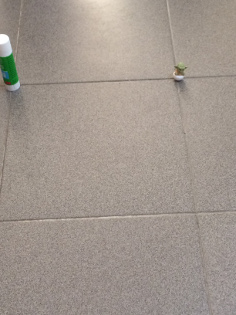
\includegraphics[width=5.0cm,trim=4 4 6 4,clip]{./images/cerchio/PiccolomanualeLibreLogo5-img2.jpg}
   \label{cer-1}
\end{figure}
\end{minipage} \hfill
\begin{minipage}{0.4\textwidth}
\begin{figure}[H]
   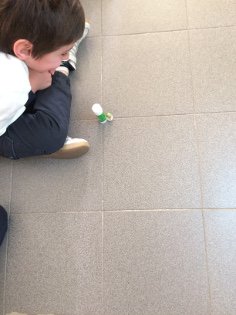
\includegraphics[width=5.0cm,trim=4 4 6 4,clip]{./images/cerchio/PiccolomanualeLibreLogo5-img3.jpg}
   \label{cer-2}
\end{figure}
\end{minipage} \hfill

Chiedo a Davide di far partire la tartaruga, percorre un tratto, ma poi non si gira, anche se le abbiamo detto di girare a destra, allora spiego che bisogna dirle di girare di 90 (gradi): i bambini osservano che la tartaruga si gira e allora... 

\vskip 1cm

\begin{minipage}{1.0\textwidth}
\begin{itemize}[itemsep=-3pt,parsep=2pt]
\item[] \hspace{8pt}FORWARD 100
\item[] \hspace{8pt}RIGHT 90   
\item[] \hspace{8pt}FORWARD 100  
\item[] \hspace{8pt}RIGHT 90     
\item[] \hspace{8pt}FORWARD 100  
\item[] \hspace{8pt}RIGHT 90     
\item[] \hspace{8pt}FORWARD 100 
\end{itemize}          	          
\end{minipage}

\vskip 1cm

Davide scrive i comandi, introduce i vari tasti e ...magia finalmente la tartaruga disegna il quadrato; intenzionalmente decido di non scrivere home, così la tartaruga può continuare a muoversi e formare quattro quadrati. È tutto questo ha già il suo fascino. Successivamente introduco una rotazione a caso della tartaruga e le chiediamo di continuare a lavorare: "che bello, sembrano le nostre cornicette"commenta Giulia; ma l'osservazione più significativa, che formula sempre Giulia, è: "Guarda, sta diventando rotondo". 

I bambini a coppie al portatile aprono LibreOffice e fanno da soli la stessa cosa che abbiamo visto insieme con interpretazioni differenti sull'ultima rotazione. 

Introduco anche il comando del colore e anche qui dopo qualche tentativo avvengono libere interpretazioni e combinazioni di colori.

\begin{minipage}{0.35\textwidth}
\begin{figure}[H]
   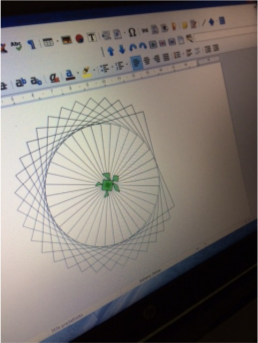
\includegraphics[width=4.0cm,trim=4 4 6 4,clip]{./images/cerchio/PiccolomanualeLibreLogo5-img4a.png}
   \label{cer-3}
\end{figure}
\end{minipage} \hfill
\begin{minipage}{0.7\textwidth}
\begin{figure}[H]
   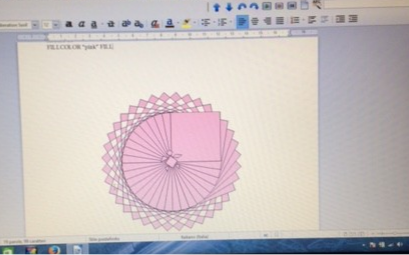
\includegraphics[width=6.0cm,trim=4 4 6 4,clip]{./images/cerchio/PiccolomanualeLibreLogo5-img4b.png}
   \label{cer-4}
\end{figure}
\end{minipage} \hfill
%\begin{minipage}{0.4\textwidth}
\begin{figure}[H]
   \centering
   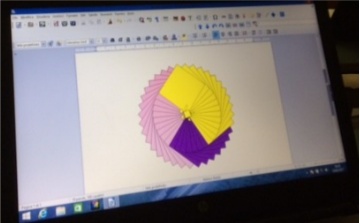
\includegraphics[width=8.0cm,trim=4 4 6 4,clip]{./images/cerchio/PiccolomanualeLibreLogo5-img4c.png}
   \label{cer-5}
\end{figure}
%\end{minipage} \hfill

Abbiamo avuto un momento di pausa e la settimana scorsa sono tornati di nuovo gli studenti con i quali abbiamo ripreso l'esperienza. Ho colto un'occasione d'oro quando è uscita la domanda: "Ma come si disegna il cerchio?" 
"Secondo voi?" ho risposto.
Sono partite le ipotesi, si sono avvicinati, ma non hanno ancora trovato la soluzione; poi, ad un certo punto, dopo che hanno intuito che right 1 poteva essere utile, una bambina ha osservato: "Con sempre right la tartaruga gira su se stessa e non si muove".

Quello che ho trovato di molto significativo in questa esperienza è che la progettazione aiuta i bambini a mobilitare e raggiungere molte competenze, per esempio destra e sinistra: in prima si dedica parecchio tempo a questo obiettivo, schede, esercizi..., forse l'attività di progettazione, come del resto affermava Papert, è più stimolante e lascia tracce indelebili nel processi di apprendimento. 

Sabato, 3 giugno

Riprendo solo oggi le fila del discorso. Il 23 maggio appunto ho voluto sperimentare la dimensione sintonica dell'apprendimento. Siamo andati in corridoio e prima abbiamo sperimentato con il corpo i comandi che abbiamo imparato a dare alla tartaruga

L'obiettivo era quello di scoprire i comandi per il cerchio, allora abbiamo per prima cosa percorso un disegno che c'è a terra nel nostro corridoio, osservando attentamente i nostri movimenti.

\begin{figure}[H]
   \centering
   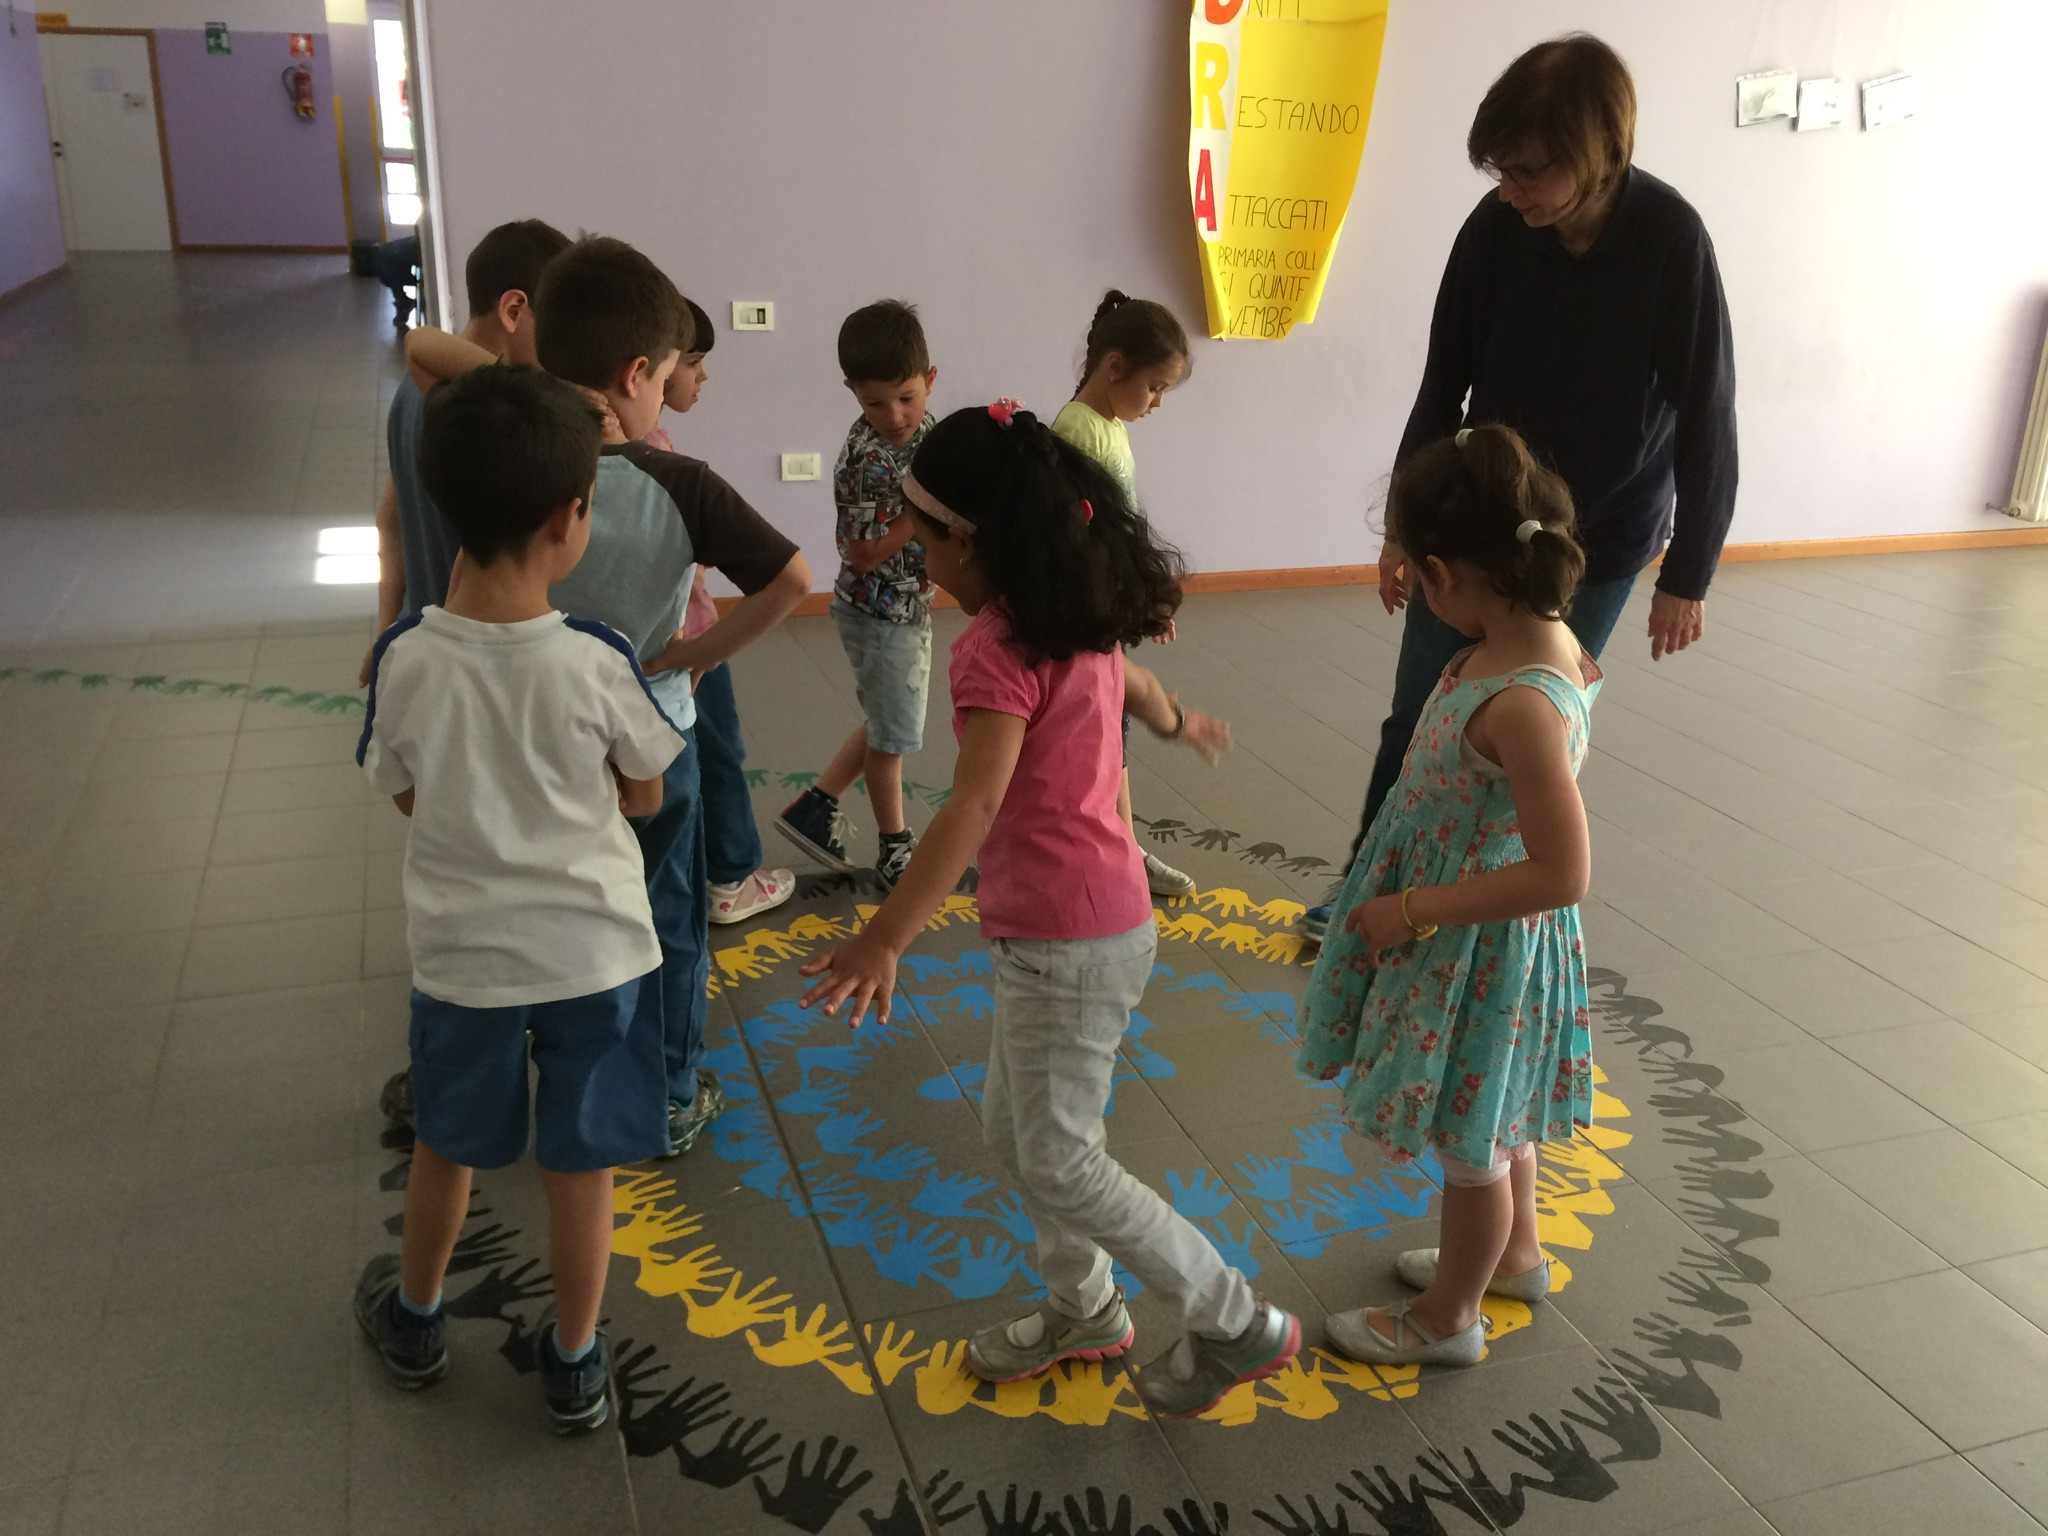
\includegraphics[width=10.0cm,trim=4 4 6 4,clip]{./images/cerchio/PiccolomanualeLibreLogo5-img5.jpg}
   \label{cer-6}
\end{figure}

Poi abbiamo abbiamo camminato sul bordo di un cerchio che si usa in educazione motoria in palestra.


\begin{minipage}{0.4\textwidth}
\begin{figure}[H]
\begin{center}
   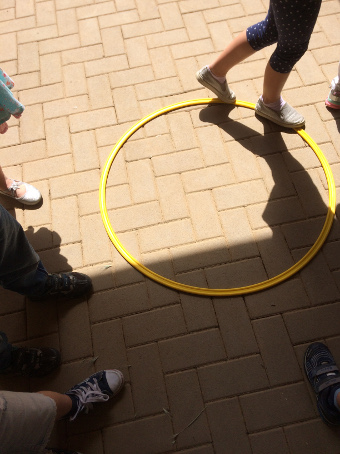
\includegraphics[width=5.0cm,trim=4 4 6 4,clip]{./images/cerchio/PiccolomanualeLibreLogo5-img6.jpg}
\end{center}
   \label{cer-7}
\end{figure}
\end{minipage} \hfill
\begin{minipage}{0.4\textwidth}
\begin{figure}[H]
\begin{center}
   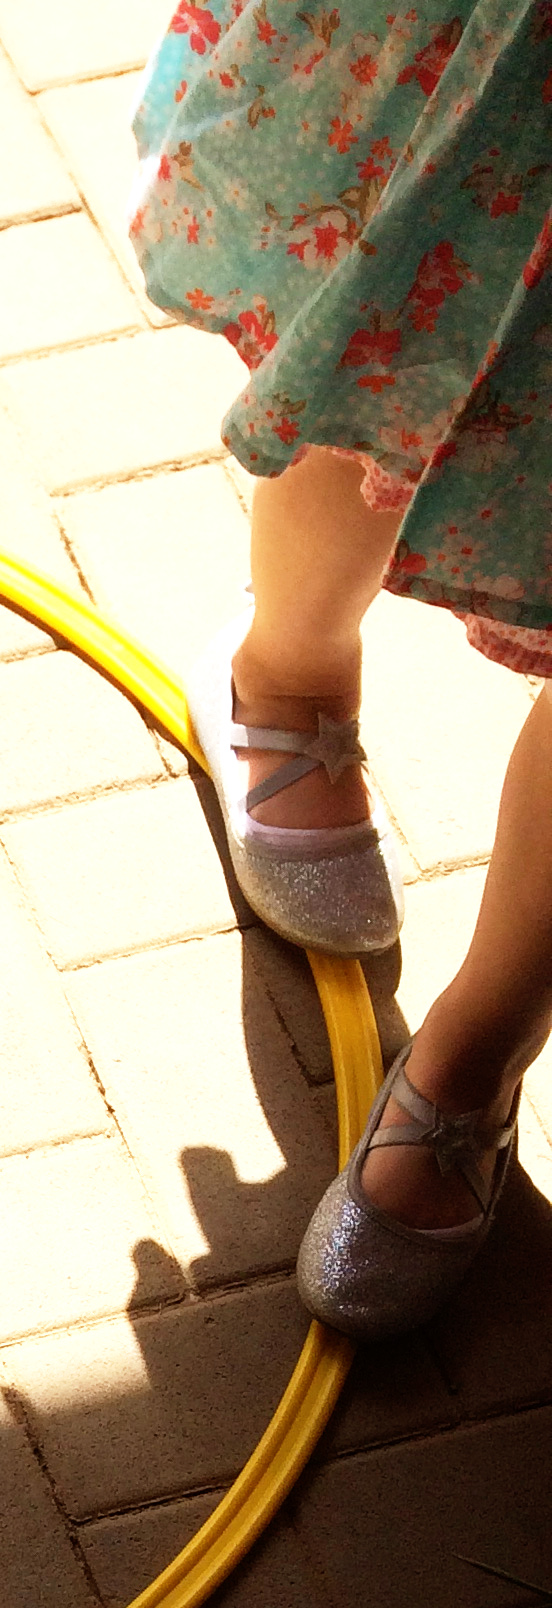
\includegraphics[width=2.3cm,trim=4 4 6 4,clip]{./images/cerchio/PiccolomanualeLibreLogo5-img7.jpg}
\end{center}
   \label{cer-8}
\end{figure}
\end{minipage} \hfill

\end{quote}

Prima di far continuare Antonella, è interessante notare nella foto a destra come la bambina cerchi di seguire la curva della circonferenza descrivendo così, con i piedi, il processo: faccio un piccolo passo e giro un poco, faccio un piccolo passo e giro un poco...

\begin{quote}

Infine..."via le calzine, tracciamo un cerchio con le orme dei nostri piedini, camminando sulla farina, come se fossimo al mare" (complice il tempo che era particolarmente soleggiato e caldo!).

\begin{minipage}{0.4\textwidth}
\begin{figure}[H]
   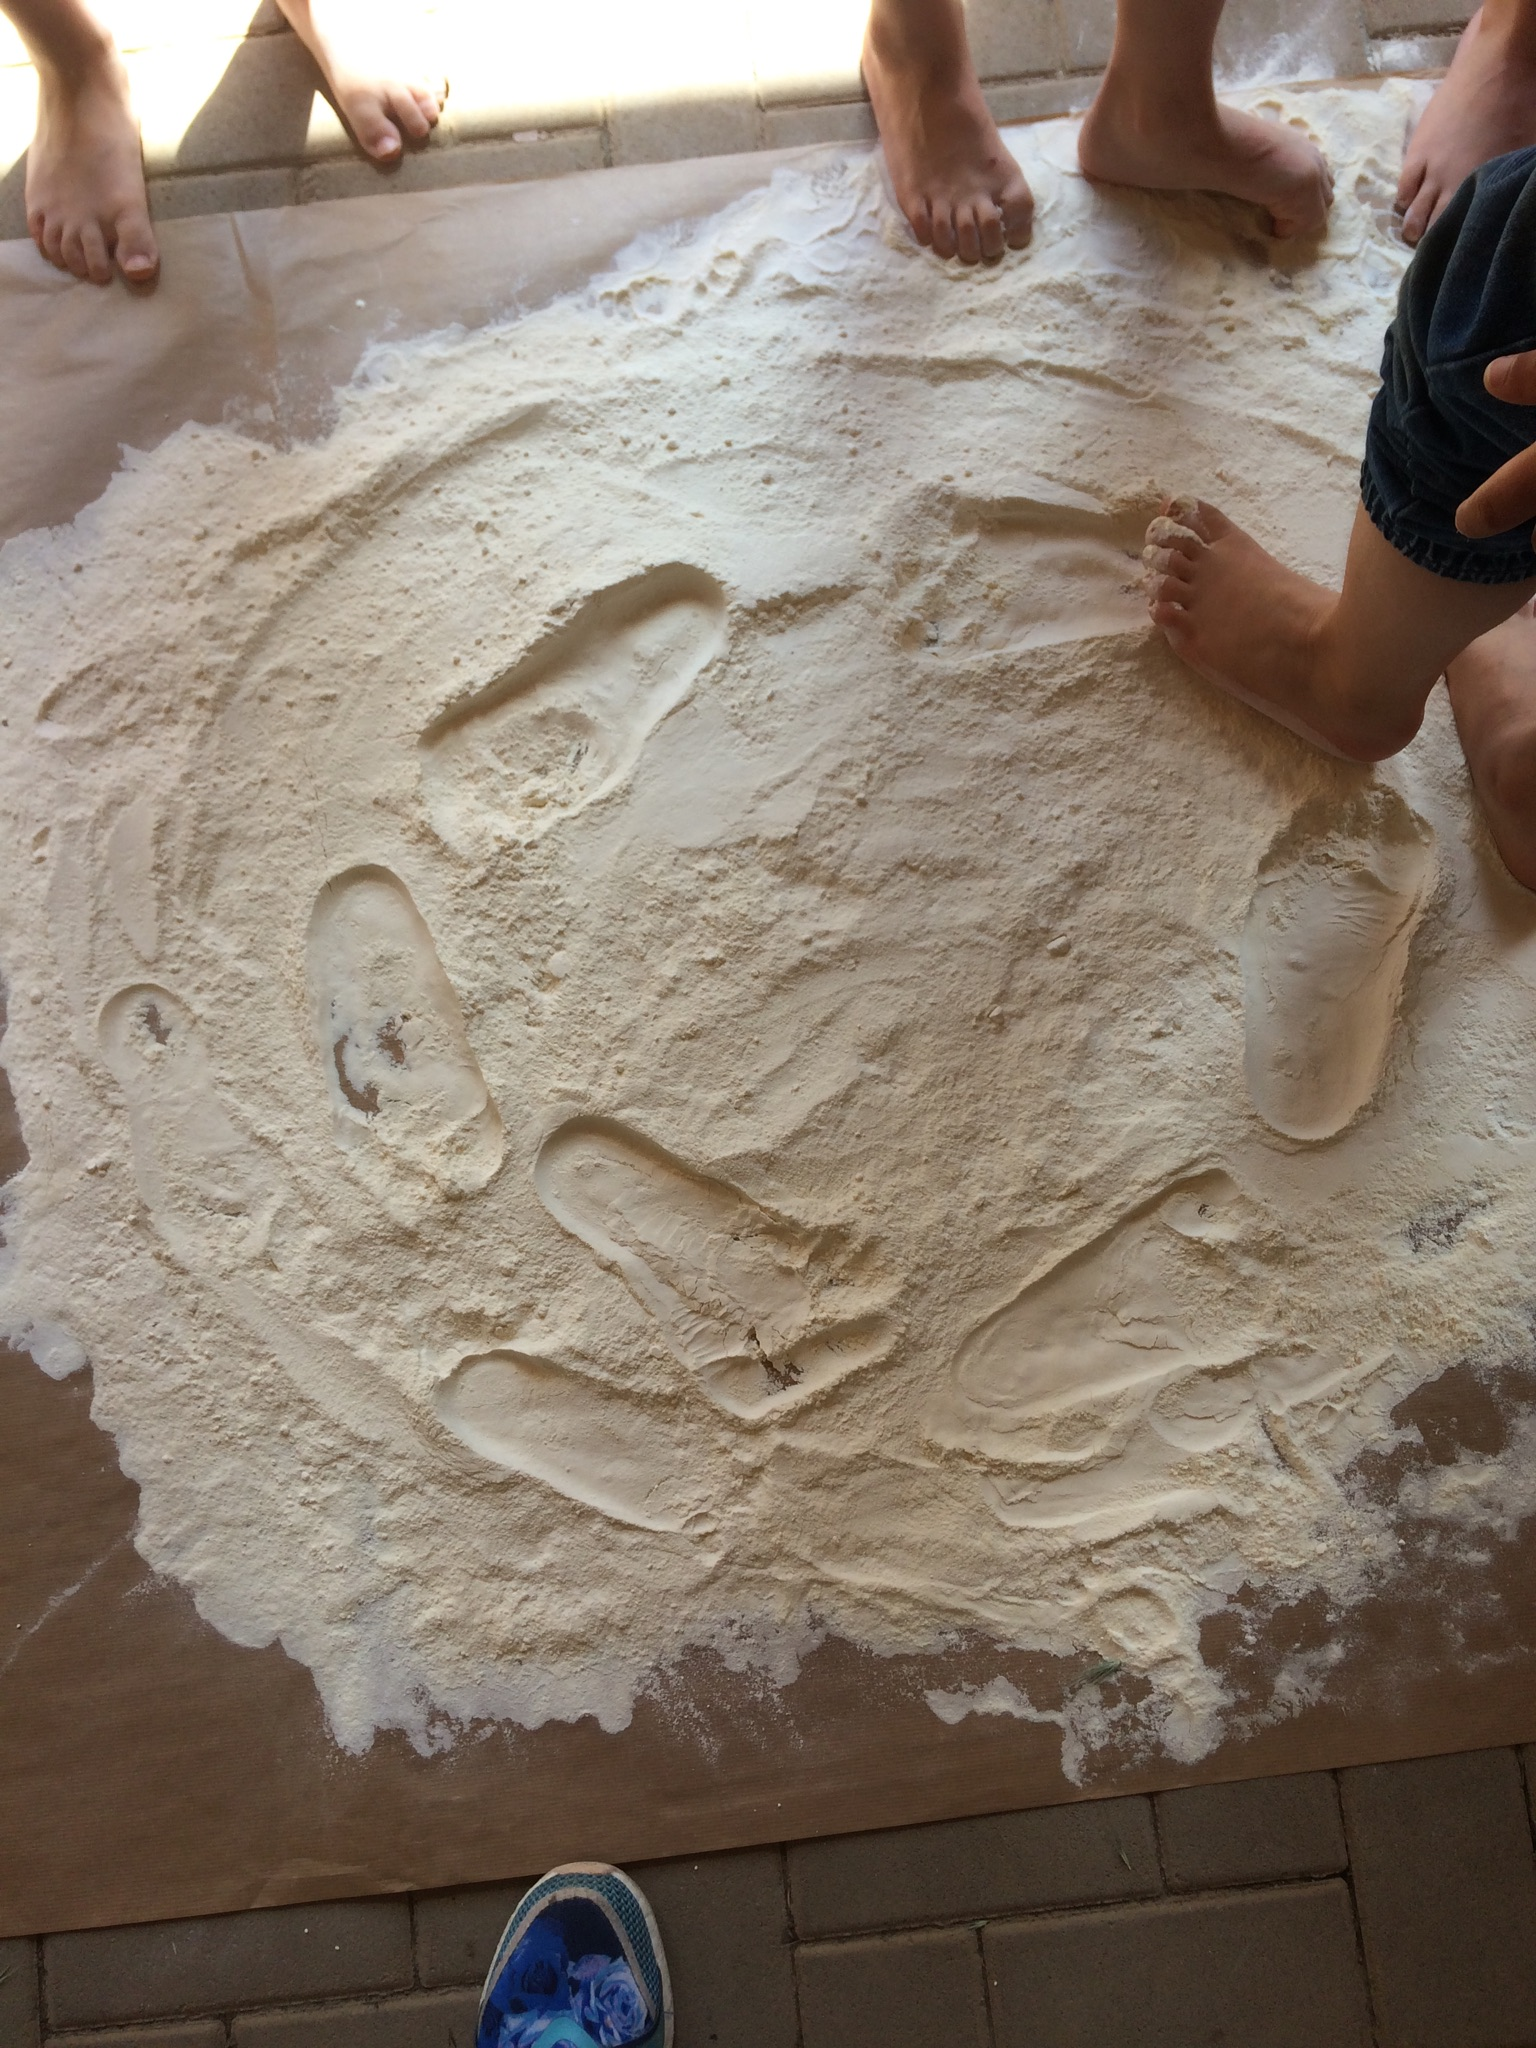
\includegraphics[width=5.0cm,trim=4 4 6 4,clip]{./images/cerchio/PiccolomanualeLibreLogo5-img8.jpg}
   \label{cer-9}
\end{figure}
\end{minipage} \hfill
\begin{minipage}{0.4\textwidth}
\begin{figure}[H]
   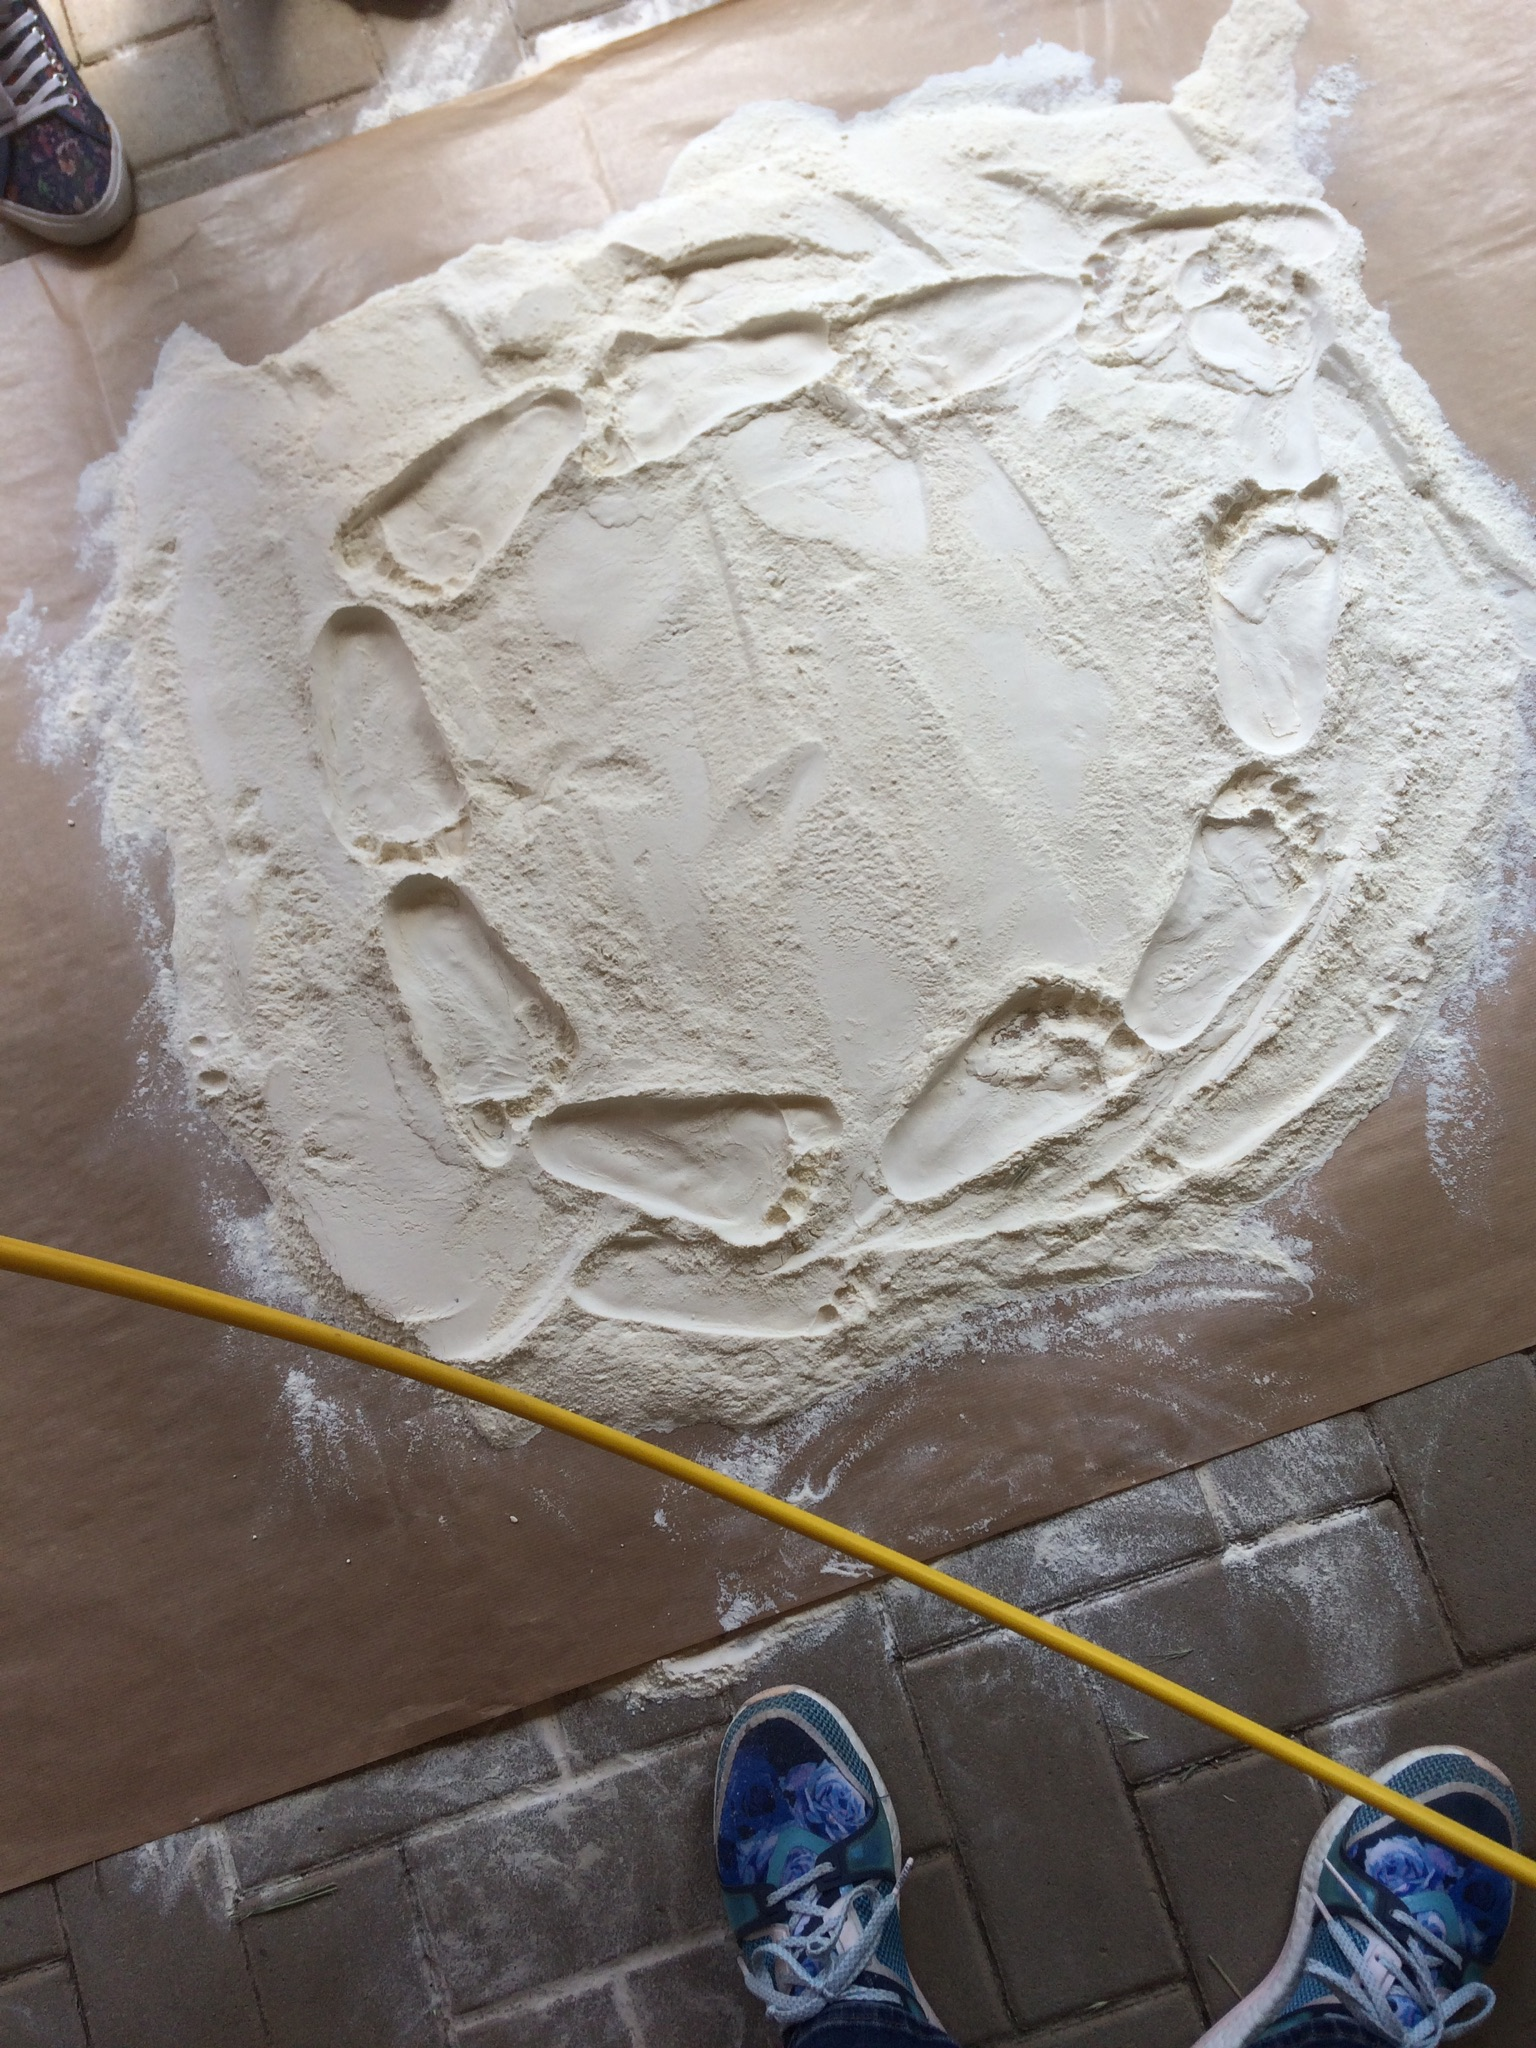
\includegraphics[width=5.0cm,trim=4 4 6 4,clip]{./images/cerchio/PiccolomanualeLibreLogo5-img9.jpg}
   \label{cer-10}
\end{figure}
\end{minipage} \hfill

Dopo l'esperienza gioiosa e coinvolgente del camminare a piedi scalzi sulla farina, c'è il momento della discussione: quali comandi dare alla tartaruga per disegnare il cerchio?

La settimana scorsa ho proposto ai bambini di usare il pc e di provare a disegnare il cerchio: usano forward e right, ma assegnano valori come 90, 40...; io suggerisco  di verificare che cosa disegna la tartaruga con le procedure scritte: procedono dunque per prove ed errori. Ben presto si rendono conto che qualcosa non va.

"Bisogna cambiare i numeri"

"Dobbiamo andare in curva"

"Bisogna continuare a fare right"

"Se facciamo sempre right, viene un punto piccolissimo".

Poi l'insight:

"Dobbiamo fare forward 1 right 1".

"Proviamo" suggerisco io

"Bisogna ripeterlo tante tante volte.

Li aiuto a scrivere, faccio finta di non sapere e di essere stanca di scrivere, per cui faccio vedere che con Ctrl+V il comando può essere ripetuto tante volte quanto vogliamo noi, per cui continuo a cliccare Ctrl+V finché loro mi dicono stop.

La tartaruga disegna e traccia un arco: è già qualcosa. Ne approfitto per introdurre repeat e chiedo quante volte devo far ripetere alla tartaruga forward1, right 1.

100...200...300 e intanto, grazie a questi tentativi, la tartaruga traccia archi sempre più ampi. Manca poco, Giovanni mi propone di scrivere 355, ma in classe ho delle ragazzine di V (la loro maestra è assente e tutti gli alunni sono stati distribuiti nelle classi) che interrompono il loro lavoro e seguono il nostro, le coinvolgo e i bambini chiedono il loro parere –  "Perché sono di V, sono più grandi di noi". Immediatamente mi rispondono 360 e finalmente la tartaruga disegna un cerchio.

\end{quote}

È affascinante come queste prime esperienze possano indurre a riflettere sul concetto di cerchio senza che se ne abbia ancora una conoscenza formale. Eppure, così facendo, si lambisce un concetto assai più avanzato di tutto ciò che i ragazzi vedranno prima della maturità, ovvero il concetto di calcolo differenziale. Tuttavia, appena essi verranno in possesso della nozione formale di circonferenza, sarà possibile tornare in Logo e riprendere il discorso attraverso il modo sintetico di produrre un cerchio, con l'istruzione CIRCLE D, dove D rappresenta il diametro del cerchio, riflettendo sulla definizione come luogo dei punti equidistanti da un dato punto. E qui si potrebbe andare oltre, partendo dall'idea di un "cerchio sbagliato", o "schiacciato", e ricorrendo alle riflessioni di Emma Castelnuovo\cite{Castelnuovo}.

\begin{quote}
Sempre un argomento di matematica, quale lo studio dei triangoli isoperimetrici con ugual base, porta a osservare quello che abbiamo sotto gli occhi. 

Il materiale è, anche questa volta, un pezzo di spago.

Per costruire dei triangoli di uguale base e uguale perimetro facciamo così: fissiamo due chiodi – siano A e B – su un tavolo su cui è disteso un foglio di carta; AB sarà la base dei nostri triangoli. Leghiamo poi gli estremi di un pezzo di spago ai due chiodi, tenendo presente che lo spago deve essere più lungo del tratto AB. Facciamo in modo, valendoci di una matita, che lo spago resti sempre ben teso e... lasciamoci guidare dalla matita.

\begin{figure}[H]
   \centering
   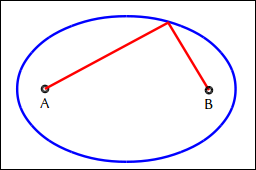
\includegraphics[width=5.0cm,trim=4 4 6 4,clip]{./images/cerchio/ellisse-emma.png}
   \label{ellisse-emma}
\end{figure}

Questa, guidata dallo spago, disegnerà sul foglio una curva a forma di ovale: è un'ellisse. I punti A e B si chiamano fuochi dell'ellisse. Dunque: i vertici dei triangoli isoperimetrici e di uguale base si trovano su un'ellisse.

Un problema di geometria ci ha condotti al disegno dell'ellisse. Con lo stesso pezzo di spago possiamo costruire un'ellisse più o meno "schiacciata", a seconda della distanza fra i punti A e B. Si può ottenere anche un cerchio, se i due punti coincidono: il cerchio, infatti, è un'ellisse particolare.    

L'ellisse, dopo averla incontrata in problemi di geometria, la ritroviamo per la strada, quando la "calpestiamo" (perché un disco segnaletico dà, come ombra, un'ellisse. Nella nostra vita convulsa raramente ci soffermiamo a osservare l'ombra di un oggetto data dai raggi del soleo da una lampadina. Ma ecco che ora un'attività di geometria ci sollecita a guardare di più ed è proprio il confronto fra l'effetto-ombra dato dai raggi del sole e quello dato da una lampada puntiforme che stimola la nostra facoltà di osservazione. 

Guardiamo, ad esempio, due matite disposte in verticale su un tavolo. Se vengono illuminate dal sole accade che anche le ombre sono parallele; se invece è una lampada che le illumina le ombre si divaricano.

Da qui lo studio matematico delle trasformazioni affini e delle trasformazioni proiettive, fino ad arrivare alla prospettiva, all'arte, a come si guarda un quadro, alla storia.

È un piccolo problema di geometria che ha stimolato a osservare e a... guardarsi intorno.

\end{quote}

Sono esperienze fisiche quella che propone Emma Castelnuovo ma non vanno considerate in contrapposizione a quelle che si possono fare con un computer, nel modo che abbiamo mostrato; che poi è il modo che suggerisce Papert attraverso il concetto di apprendimento sintonico. 

Purtroppo l'avvento del nuovo viene solitamente vissuto in contrapposizione al vecchio, generando l'usuale dicotomia integrati-apocalittici. È il tempo a risolvere solitamente ciò che la saggezza potrebbe evitare subito, con molto maggiore profitto. Quella da promuovere è quindi una visione integrata, dove si fa ricorso a tutti i mezzi possibili, tradizionali e moderni, manuali e virtuali, per raggiungere gli obiettivi didattici in una prospettiva più ampia e completa possibile.


\section{... high ceiling}

Fin qui abbiamo esplorato "il tondo" dal basso, dal \textit{low floor} di Papert, almeno in parte. Molto altro potrebbe essere aggiunto, ma ora, per rifarsi al quesito iniziale, proviamo a muoverci verso l'alto per vedere dove si possa trovare l'\textit{high ceiling}. Si tratta di un quesito che è emerso per esempio recentemente durante un incontro con un nutrito gruppo di animatori digitali, dove ci si poneva la domanda: ma si può fare il \textit{coding} anche negli anni successivi, alle scuole superiori? Molti sostenevano di no, ritenendo che si trattasse di pratiche troppo banali.

Riprendiamo le parole di Papert.

\begin{quote}

Il bambino che ha disegnato il cerchio con la Tartaruga non ha imparato qualcosa sul formalismo dell'analisi, per esempio che la derivata di $x^n$ è $nx^{n-1}$, ma qualcosa sul suo impiego e sul suo significato. Infatti il codice per disegnare il cerchio con la Tartaruga conduce a un formalismo alternativo di quelle che sono tradizionalmente chiamate "equazioni differenziali" ed è un veicolo efficace delle idee che soggiaciono al differenziale. Questo è il motivo per cui si possono capire così tante cose con la Tartaruga; il  codice del cerchio rappresenta un'analogia intuitiva dell'equazione differenziale, un concetto che appare in quasi tutti gli esempi di matematica applicata tradizionale.

La potenza del calcolo differenziale risiede molto nella capacità di descrivere le variazioni in base a ciò che accade nelle loro immediate vicinanze. È questa caratteristica che ha consentito a Newton di descrivere il moto dei pianeti. Via via che questi tracciano l'orbita, sono le condizioni locali nel luogo dove si trova il pianeta che determinano il suo prossimo passo. Nelle nostre istruzioni della Tartaruga, FORWARD 1 RIGHT 1, ci si riferisce solo al luogo dove si trova la Tartaruga e a quello dove si troverà il momento dopo. Questo è quello che rende differenziale un'equazione. In ciò non vi è alcun riferimento a luoghi remoti rispetto al percorso. La Tartaruga vede il cerchio cammin facendo, nell'immediata vicinanza, ed è cieca rispetto a tutto il resto che si trova più lontano. Questa proprietà è così importante che i matematici hanno un nome per essa: la geometria della Tartaruga è "intrinseca". Lo spirito della geometria differenziale intrinseca si palesa quando si considerano i diversi modi di concepire una curva, ad esempio il  cerchio. Per Euclide la caratteristica che definisce il cerchio è la distanza costante dei suoi punti da un altro punto, il centro, che però non fa parte di esso. Nella geometria di Cartesio, in questo caso più similmente a Euclide, i punti del cerchio sono caratterizzati dalla loro distanza rispetto a qualcos'altro, vale a dire dai due assi perpendicolari delle coordinate. Così, per esempio, un cerchio è definito da:

\begin{equation}
(x-a)^2+(y-b)^2= R^2
\end{equation}

Nella geometria della Tartaruga un cerchio è definito dal fatto che questa continua a ripetere uno stesso atto: FORWARD un poco, GIRA un poco. Questa ripetizione garantisce che la curva abbia "curvatura costante", dove si stabilisce di quanto si deve girare ad ogni passo.

La geometria della Tartaruga appartiene ad una famiglia di geometrie che godono di proprietà assenti in quelle euclidea e cartesiana. Queste sono le geometrie differenziali che si sono sviluppate a partire da Newton e che hanno reso possibile gran parte della fisica moderna. Abbiamo osservato come quello delle equazioni differenziali sia il formalismo che ha consentito alla fisica di descrivere  il moto di una particella o di un pianeta. Nel capitolo 5 [NdR: di Minstorms], dove descriveremo questo fatto con maggiori dettagli, vedremo come questo sia anche il formalismo appropriato per descrivere il moto di un animale oppure l'evoluzione di un'economia. E arriveremo anche a capire che non è un coincidenza il fatto che la geometria della Tartaruga sia collegata sia all'esperienza di un bambino che alle principali conquiste della fisica, in quanto, la visione del moto di un bambino, sebbene meno precisa nella forma, condivide la struttura matematica dell'equazione differenziale con le leggi del moto di un pianeta che gira intorno al sole o quelle delle falene che girano introno alla fiamma di una candela. E la Tartaruga non è ne più ne meno che la ricostruzione in forma computazionale intuitiva del nucleo qualitativo di questa struttura matematica. Quando torneremo su queste idee  nel capitolo 5, vedremo come la geometria della Tartaruga apra le porte alla comprensione intuitiva dell'analisi, della fisica e della modellazione matematica così come viene impiegata nelle scienze biologiche e sociali.

\end{quote}

Prendiamo quindi le mosse dal riferimento di Papert alla fisica di Newton, rifacendosi dai principi della dinamica e dalla legge di gravitazione universale.

\subsection{La visione analitica classica}

Poniamo il problema in maniera generale. Non potrà essere questa l'impostazione proposta a scuola, perché occorrono conoscenze matematiche superiori, ma qui ci serve per inquadrare e comprendere correttamente la questione.

Affrontiamo il problema di due corpi che siano isolati da perturbazioni esterne. Ad esempio quello di un satellite che gira intorno alla terra o di una cometa che gira attorno a un pianeta. Il moto di questi corpi è governato dalla legge di gravitazione universale di Newton:

\begin{equation} \label{eq:newton}
\mathbf{F}_{Mm}=-\frac{GMm}{r^2}\frac{\mathbf{r}}{r}
\end{equation}

Dove $\mathbf{F}_{Mm}$ è la forza, $G$ la costante di gravitazione universale, pari a $6.67\times 10^{-11}$ $(Newton \times metri^2 / Kg^2) $, $M$ è la massa del pianeta, $m$ la massa del satellite, $\mathbf{r}$ la distanza fra i baricentri dei due corpi e dove, ricordiamo, il grassetto si denota per indicare la naturale vettoriale di una quantità. Quindi in questo specifico caso, poiché il nostro ragionamento si svolge tutto in due dimensioni, la forza $\mathbf{F}_{Mm}$ e la distanza $\mathbf{r}$ sono vettori con due componenti: una lungo $x$ e l'altra lungo $y$. 

Ma cosa vuol dire in pratica che "il moto dei corpi è governato dalla legge di gravitazione"? Significa che, per individuare il moto di un corpo, dobbiamo applicare il II principio della dinamica, secondo il quale:

\begin{equation} \label{eq:fma}
\mathbf{F}=m\mathbf{a}
\end{equation}

Dove $\mathbf{F}$ è la forza applicata al corpo di massa $\mathbf{F}$ e $\mathbf{a}$ è l'accelerazione impressa al corpo in virtù di tale forza. Lo scopo di queste relazioni è quello di consentire la determinazione del moto dei corpi a partire da predeterminate condizioni iniziali. Per fare questo occorre riscrivere l'equazione \ref{eq:fma} tenendo conto della forza data nell'equazione \ref{eq:newton}:

\begin{equation}
-\frac{GMm}{r^2}\frac{\mathbf{r}}{r}=m\mathbf{a}
\end{equation}

Risolvere questa equazione significa in primo luogo ricavare l'accelerazione $\mathbf{a}$:

\begin{equation} \label{eq:acc}
\mathbf{a}=-\frac{GM}{r^2}\frac{\mathbf{r}}{r}
\end{equation}

e da questa derivare l'andamento nel tempo della velocità e quindi dell'accelerazione, tenendo conto che:

\begin{equation}
\mathbf{a}=\frac{d^2\mathbf{r}}{dt^2}
\end{equation}

ovvero

\begin{equation}
\mathbf{v}=\frac{d\mathbf{r}}{dt},\mathbf{a}=\frac{d\mathbf{v}}{dt}
\end{equation}

È qui che ci dobbiamo fermare, perché siamo di fronte a equazioni dove non appaiono le grandezze incognite, ma le derivate di tali grandezze rispetto a un'altra variabile, il tempo in questo caso. In particolare, l'equazione \ref{eq:acc} è un'equazione differenziale del II ordine perché fornisce un'espressione per l'accelerazione, ovvero la derivata seconda della posizione rispetto al tempo.  Ci dobbiamo fermare perché la soluzione delle equazioni differenziali non rientra nell'orizzonte contemplato dai programmi della scuola secondaria. Di fatto l'approfondimento che ci possiamo permettere è assai limitato. L'apprendimento della fisica nella scuola si limita per di più alla memorizzazione di alcune formule e all'esecuzione di qualche esercizio, con procedimenti che la maggioranza degli studenti assimilano in maniera meccanica e effimera, senza realmente comprendere l'essenza dei concetti e tanto meno senza recepire il benché minimo sentore del "pensiero fisico", come del resto del "pensiero matematico". I risultati si vedono dal fatto che nella cittadinanza sopravvivono solo brandelli di pensiero scientifico, un pensiero che non ha quasi nulla a che vedere con l'avere imparato a memoria $F=ma$ una volta nella vita, giusto per superare un'interrogazione.

Ci colpisce tuttavia il fatto che di calcolo differenziale abbiamo già parlato, e che lo abbiamo fatto addirittura trovandoci al \textit{low floor}, dove stavamo parlando di attività da fare con allievi assai più piccoli! Lì avevamo descritto, anzi Papert aveva descritto, il concetto come un processo locale: il bambino (o la Tartaruga) che produce un cerchio preoccupandosi solo di fare un passo e girare, senza alcuna nozione esplicita e sintetica del concetto di cerchio. Ebbene questa è proprio la descrizione verbale di un'equazione differenziale, dove anziché esprimere delle quantità in funzione di altre si esprimono le loro variazioni, le quali sono sempre inerentemente locali.

\subsection{Fisica computazionale}

Affrontiamo quindi il problema espresso dall'equazione \ref{eq:acc} in maniera computazionale.  Riscriviamo l'equazione così:

\begin{equation}
\frac{d^2\mathbf{r}}{dt^2}=-\frac{GM}{r^2}\frac{\mathbf{r}}{r}
\end{equation}

O volendo così (ognuno faccia riferimento alla versione che preferisce):

\begin{equation}
\frac{d}{dt}\frac{d\mathbf{r}}{dt}=-\frac{GM}{r^2}\frac{\mathbf{r}}{r}
\end{equation}

E affrontiamolo nel seguito come avevamo fatto con il cerchio alla maniera di Papert, dove si faceva un piccolo passo per volta e poi si girava di un po', e via di seguito. Anche qui facciamo un piccolo passo per volta. 

\subsection{Le condizioni iniziali}

Ma prima di tutto: a partire da dove e in quale direzione dobbiamo fare il passo? Ecco questo è un primo concetto fondamentale del procedimento di conoscenza fisica: la determinazione delle condizioni iniziali, o delle "condizioni al contorno". Qui possiamo subito osservare come, ponendo il problema in termini computazionali anziché analitici, l'allievo sia costretto a misurarsi concretamente con il  concetto basilare di condizione al contorno e in una maniera per lui perfettamente comprensibile. Nella fisica convenzionalmente insegnata al liceo questo concetto non appare o, al più, compare in un forma astratta che ben difficilmente lascerà qualche traccia nella mente del giovane. Orbene, il punto di partenza rappresenta la condizione iniziale della posizione, che richiederà che venga fissato un sistema di riferimento, sotto forma di coordinate $(x_0,y_0)$ dell'origine di un riferimento cartesiano, e una posizione iniziale $(x,y)$ del corpo. Qui verrà presa una decisione anch'essa di natura fisica: essendosi posti nella condizione di studiare le orbite di singoli corpi intorno a un pianeta molto più grande, potremo assumere che questo stia fermo e sarà quindi naturale far coincidere il centro $(x_0,y_0)$ del sistema con il baricentro di questo. Così facendo avremo determinato la condizioni iniziale del vettore posizione $\mathbf{r}$ attraverso le due coppie di coordinate $(x_0,y_0)$ e $(x,y)$. Poi dobbiamo decidere la dimensione del passo e in che direzione compierlo. Questo lo possiamo fare se sappiamo la velocità nel punto in cui ci troviamo. Potrebbe essere zero se immaginiamo semplicemente di lasciar cadere il corpo verso la terra, ma sarà invece un valore preciso se si tratterà di imprimere la giusta velocità iniziale a un satellite o a una cometa, affinché questi percorrano le orbite che ci aspettiamo. La velocità nel punto del primo passo è la velocità iniziale e la direzione sarà determinata attraverso la reciproca dimensione delle due componenti, lungo $x$ e $y$, rispettivamente. Dopodiché, la dimensione del passo verrà determinata a partire dalla relazione $spazio = velocit\grave{a} \times tempo$ ,  che caratterizza il concetto di velocità. In pratica, dal punto di vista computazionale, ovvero di istruzioni da impartire a un computer, dovremo scrivere qualcosa del genere

\begin{equation} \label{eq:pos}
\begin{array}{ll}
\textrm{XPOS}=\textrm{XPOS}+\textrm{XVEL}*\textrm{Dt}\\
\textrm{YPOS}=\textrm{YPOS}+\textrm{YVEL}*\textrm{Dt}\\
\end{array}
\end{equation}

Dove XVEL e YVEL rappresentano le componenti della velocità e Dt l'intervallo di tempo su cui abbiamo deciso di aggiustare il passo. Prima di commentare quest'ultimo elemento, per coloro che non avessero mai visto una scrittura del genere, diciamo che questo è uno dei modi per alterare – incrementare in questo caso – una variabile. In generale, scrivere $a=a+b$ significa prendere la somma dei valori di $a$ e $b$ e attribuire questo risultato alla variabile $a$. È un modo quindi per aggiornare il valore di una variabile: a destra del segno di $=$ si usa il vecchio valore di $a$, a sinistra c'è quello nuovo attribuito in base all'operazione fatta. Detto questo, finiamo di commentare il fattore Dt. Questo rappresenta l'intervallo di tempo nel quale viene percorso il tratto a quella velocità. Deve essere piccolo perché sennò non si può ragionevolmente accettare che la velocità sia constante in quel tratto. Piccolo quanto? 

\subsection{The art of scientific computing}

La risposta onesta è: bisogna vedere... Non esattamente soddisfacente come risposta per una scienza (un tempo) ritenuta "esatta". Esiste un testo fondamentale per chiunque si sia occupato o si occupi di calcolo scientifico, pubblicato la prima volta nel 1986: Numerical Recipes – The Art of Scientific Computing\cite{Press}. Quello del calcolo scientifico non è un mondo esatto. Sembra un paradosso: laddove le scienze esatte sposano la tecnologia si parla di "arte del calcolo scientifico". In parte perché ci sono metodi matematici estremamente sensibili ad ogni piccola variazione dei dati, che in certi contesti conducono all'impossibilità di risolvere problema, e in parte perché la rappresentazione in bit dei numeri è solo un'approssimazione della loro nozione matematica, questa sì esatta. Non solo, lo stesso identico calcolo eseguito su computer diversi può dare risultati differenti, come abbiamo visto nel capitolo precedente, perché non è identico l'insieme dei processi con i quali i computer manipolano l'imperfetta rappresentazione dei numeri.

Tornando alla questione dell'intervallino di tempo Dt, anch'essa dipende molto dal contesto. Il compromesso è un po' questo: se si fanno passi lunghi allora il calcolo procede veloce ma si rischia di sbagliare molto, in particolare quando la velocità cambia apprezzabilmente fra un passo e l'altro; per sbagliare meno occorre scegliere passi più brevi e quanto più questi sono brevi, tanto più il calcolo sarà accurato. Però anche qui fino a un certo punto, perché se gli intervalli diventano brevissimi si possono avere problemi di precisione nella rappresentazione dei numeri e quindi i conti possono nuovamente sballare, oltre a rischiare di dilatare inutilmente i tempi di calcolo, se non a renderli ingestibili.

Perché tutte queste considerazioni che possono parere anche esageratamente tecniche per il nostro contesto? Da un lato per tentare di rimettere al centro la complessità e la ricchezza del pensiero computazionale, che finisce con l'essere polverizzato in un discorso pubblico banale e partigiano, strapazzato nelle diatribe fra fazioni di apocalittici e integrati, o di "umanisti" e "scientifici". A proposito di quest'ultima dicotomia vorrei dire che chi vi crede tradisce allo stesso tempo sia la visione umanistica che quella scientifica, perché una vera visione umanistica certamente comprende e valorizza il pensiero scientifico. Il pensiero scientifico è umanistico, invece v'è ne poco in giro. Dall'altro perché questa complessità fornisce un terreno adatto per un approccio alla conoscenza di natura laboratoriale, che è quello che di fatto vivono il ricercatore, l'artista o l'artigiano, quando si misurano con la realtà nei rispettivi modi e con i rispettivi strumenti. Le incertezze del calcolo scientifico non devono certamente essere rovesciate sugli allievi come si fa nell'approccio disciplinare classico, bensì devono essere tenute presenti per essere eventualmente approfondite, in misura adeguata, qualora i loro effetti si presentino nel corso delle esplorazione.

Il codice nella formula \ref{eq:pos}, se rieseguito ripetutamente, disegna la traiettoria del corpo per incrementi successivi, che è proprio quello che desideriamo. Il problema tuttavia è che ci occorre conoscere la velocità in ogni punto della traiettoria ma noi questa informazione non ce l'abbiamo; soprattutto non abbiamo niente che leghi la grandezza velocità alla legge di gravitazione (Eq. \ref{eq:acc}), che è tutto ciò che sappiamo. In realtà nell'equazione \ref{eq:acc} abbiamo l'accelerazione, che rappresenta la variazione della velocità. Quindi quello che ci occorre è un passaggio simile a quello che nel codice \ref{eq:pos} ci è servito per ricostruire il percorso. Dobbiamo cioè ricostruire l'andamento della velocità per incrementi successivi:

\begin{equation} \label{eq:vel}
\begin{array}{ll}
\textrm{XVEL}=\textrm{XVEL}+\textrm{XACC}*\textrm{Dt}\\
\textrm{YVEL}=\textrm{YVEL}+\textrm{YACC}*\textrm{Dt}\\
\end{array}
\end{equation}
Dove XACC e YACC rappresentano le componenti dell'accelerazione lungo le direzioni degli assi cartesiani X e Y. Questa  ce l'abbiamo perché è proprio la legge di gravitazione \ref{eq:acc} a darcela, che scissa nelle due componenti risulta:

\begin{equation}
\begin{array}{ll}
a_x=-\frac{GM}{r^2}\frac{r_x}{r}\\
\\
a_y=-\frac{GM}{r^2}\frac{r_y}{r}\\
\end{array}
\end{equation}

che rappresentiamo nel codice LibreLogo (vedi dopo) in questa forma:

\begin{equation}
\begin{array}{ll}
\textrm{XACC}=\textrm{GG} / \textrm{R2} * \textrm{DX} / \textrm{R}\\
\textrm{YACC}=\textrm{GG} / \textrm{R2} * \textrm{DY} / \textrm{R}\\
\end{array}
\end{equation}

Letto così può parere complesso rispetto a quanto abbiamo visto ora. Certo, non stiamo facendo un corso di fisica ma non è questo il punto. L'importante è riconoscere i blocchi principali per afferrare i concetti importanti, intravedendo il nesso con il caso (apparentemente) più semplice del cerchio che abbiamo raccontato  al \textit{low floor}. 

Prima descriviamo l'algoritmo con un pseudocodice, ovvero un codice informale che non può essere eseguito nel computer ma che serve a facilitare la comprensione degli algoritmi, scritto tenendo conto solo dei passaggi fondamentali e omettendo tutti i particolari che invece sono necessari alla macchina per potere eseguire il programma. Rammentiamo che i programmi in LibreLogo si scrivono anteponendo le procedure, in modo che, ogni volta che una di queste sia invocata, il suo codice sia già stato "letto" dalla tartaruga. Quindi il pseudocodice\footnote{Il pseudocodice è una sorta di linguaggio che sta à metà fra un vero linguaggio di programmazione, che può essere interpretato dal computer, e il linguaggio naturale. Le sue istruzioni non possono essere eseguite nella macchina ma servono a dare un'idea della struttura fondamentale di un algoritmo. In questi esempi abbiamo lasciato le pseudostruzioni in inglese, considerato che in tutto questo ambito la lingua di riferimento è l'inglese. Del resto il significato è intuitivo. Aggiungiamo solo che il costrutto "\textbf{while} condizione \textbf{do} istruzioni \textbf{end}" esprime un ciclo, dove le istruzioni comprese fra \textbf{do} e \textbf{end} vengono ripetute fintantoché risulta vera la condizione espressa fra \textbf{while} e \textbf{do}, che nel nostro caso è "orbita non è chiusa". Alla prima ripetizione in cui l'orbita risulta chiusa il ciclo si interrompe.} che segue si riferisce al cosiddetto programma principale che, nel listato completo successivo inizia a partire dall'istruzione n. 134.

\vskip 1cm

%https://en.wikibooks.org/wiki/LaTeX/Algorithms
\begin{algorithm}[H]
 \KwData{Dati del sole e del corpo orbitante, condizioni iniziali}
 \KwResult{Orbita del corpo}
 \While{orbita non è chiusa}{
  calcola prossimo punto con legge di gravitazione\;
  disegna prossimo punto\;
  scrive su file coordinate, velocità, accelerazioni nel prossimo punto }
 \caption{Pseudocodice per il calcolo dell'orbita di un corpo intorno al sole}
\end{algorithm}

\vskip 1cm

Messo così non siamo molto lontani dal codice che esprimeva il cerchio alla Papert:

\vskip 1cm

\begin{minipage}{1.0\textwidth}
\begin{itemize}[itemsep=-3pt,parsep=2pt]
\item[] \hspace{8pt}REPEAT [ FORWARD 1 RIGHT 1 ]   
\end{itemize}          	          
\end{minipage}

\vskip 1cm

che in sostanza diceva\footnote{Qui abbiamo usato la variante "\textbf{while} \textbf{do} istruzioni \textbf{end}" senza condizione, che produce una ripetizione del ciclo all'infinito.}

\vskip 1cm

\begin{algorithm}[H]
 \While{}{
   disegna prossimo punto\;}
 \caption{Pseudocodice per il calcolo della circonferenza}
\end{algorithm}

\vskip 1cm

Cos'hanno in comune di importante il codice per disegnare l'orbita di un corpo celeste e quello per disegnare il cerchio? Il fatto di farlo esclusivamente in base a valutazioni locali, senza impiegare la conoscenza esplicita dell'ellisse in un caso e del cerchio nell'altro, ovvero senza utilizzare le equazioni delle rispettive curve. In termini matematici, questa "valutazione locale" non vuol dire altro che risolvere l'equazione differenziale che descrive un certo fenomeno. Torneremo dopo su questo, ora era necessario solo cercare di cogliere questa corrispondenza matematica, prima di tuffarsi un poco nei particolari del codice per l'orbita di un corpo reale, che per la sua particolare natura richiede una serie di accorgimenti, i quali spostano considerevolmente in alto l'\textit{high ceiling}. Forse anche troppo, in media, per  una scuola secondaria, ma non è affatto escluso, che in una situazione laboratoriale, un insegnante e degli studenti in gamba vi si possano arrampicare. L'esempio è comunque utile per mettere in luce vari aspetti che mostrano come l'approccio computazionale consenta di avvicinarsi in maniera molto più concreta allo studio dei fenomeni fisici, sotto vari aspetti, e anche come il calcolo scientifico sia ben lontano da quel banale determinismo che taluni, intrappolati in una miope visione dicotomica fra \textit{humanities} e scienza, vorrebbero far credere. Tant'è che l'espressione "\textit{art of scientific computing}" è comune e pertinente. In ultimo, l'esempio è istruttivo anche per mostrare come non siano necessari strumenti sofisticati per realizzare compiti che possono essere anche considerevolmente complessi, dal punto di vista scientifico.  Insomma Logo non è limitato al disegno delle casette. E per questo che abbiamo aggiunto, ad esempio, la scrittura su di un file dei dati calcolati nel processo –  posizioni velocità e accelerazioni – per mostrare che LibreLogo può anche essere considerato un sistema per eseguire calcolo, vero e proprio, e non solo per fare un po' di grafica. 

Nelle pagine successive riportiamo il listato del codice, ampiamente commentato, per il caso della cometa di Halley che orbita intorno al sole. Aggiungiamo poi qualche considerazione per approfondire alcuni aspetti più rilevanti. La sorgente del codice, in formato ODT, la mettiamo a disposizione in un file a parte\footnote{Il codice è accessibile pressol'URL http://iamarf.ch/unifi/Halley-RK-4-AU-90-distribuibile.odt}, in maniera che possa essere eseguito da tutti. 

\vskip 1cm

%https://en.wikibooks.org/wiki/LaTeX/Source_Code_Listings
\lstset{literate=
  {á}{{\'a}}1 {é}{{\'e}}1 {í}{{\'i}}1 {ó}{{\'o}}1 {ú}{{\'u}}1
  {Á}{{\'A}}1 {É}{{\'E}}1 {Í}{{\'I}}1 {Ó}{{\'O}}1 {Ú}{{\'U}}1
  {à}{{\`a}}1 {è}{{\`e}}1 {ì}{{\`i}}1 {ò}{{\`o}}1 {ù}{{\`u}}1
  {À}{{\`A}}1 {È}{{\'E}}1 {Ì}{{\`I}}1 {Ò}{{\`O}}1 {Ù}{{\`U}}1
  {ä}{{\"a}}1 {ë}{{\"e}}1 {ï}{{\"i}}1 {ö}{{\"o}}1 {ü}{{\"u}}1
  {Ä}{{\"A}}1 {Ë}{{\"E}}1 {Ï}{{\"I}}1 {Ö}{{\"O}}1 {Ü}{{\"U}}1
  {â}{{\^a}}1 {ê}{{\^e}}1 {î}{{\^i}}1 {ô}{{\^o}}1 {û}{{\^u}}1
  {Â}{{\^A}}1 {Ê}{{\^E}}1 {Î}{{\^I}}1 {Ô}{{\^O}}1 {Û}{{\^U}}1
  {œ}{{\oe}}1 {Œ}{{\OE}}1 {æ}{{\ae}}1 {Æ}{{\AE}}1 {ß}{{\ss}}1
  {ű}{{\H{u}}}1 {Ű}{{\H{U}}}1 {ő}{{\H{o}}}1 {Ő}{{\H{O}}}1
  {ç}{{\c c}}1 {Ç}{{\c C}}1 {ø}{{\o}}1 {å}{{\r a}}1 {Å}{{\r A}}1
  {€}{{\euro}}1 {£}{{\pounds}}1 {«}{{\guillemotleft}}1
  {»}{{\guillemotright}}1 {ñ}{{\~n}}1 {Ñ}{{\~N}}1 {¿}{{?`}}1
}
\lstset{extendedchars=true, numbers=left,basicstyle=\scriptsize} 
\begin{lstlisting}[frame=single]  % Start your code-block
; Copyright 2018 Andreas Robert Formiconi

; Programma distribuito alle condizioni della GNU General Public License

; Questo programma è Software Libero (Free Software): può essere
; ridistribuito e modificato nei termini della GNU General Public 
; License pubblicata dalla Free Software Foundation, nella versione 3 o 
; una delle successive. Il testo della licenza è accessibile in 
; <https://www.gnu.org/licenses/licenses.it.html>.

; Calcolo dell'orbita di un corpo celeste intorno al sole mediante 
; integrazione numerica delle equazioni del moto governate dalla legge 
; di gravitazione di Newton.  Il problema è posto in due dimensioni e 
; assume che non vi siano perturbazioni da parte di altri corpi. 
; Il codice è aggiustato per risolvere il caso di un'orbita fortemente 
; eccentrica come quello della cometa di Halley.

; La Tartaruga gioca il ruolo della cometa Il pianeta sta al centro, 
; che in LibreLogo ha coordinate [297.89,421.11] dove la unità di 
; misura è il "punto" (p).  Lo spazio della pagina è 
; (pagg. 63-65 del Piccolo Manuale di LibreLogo)

;    [0, 0] --------  [596, 0]
;      |                   |
;      |                   |
;      |                   |
;      |                   |
;      |                   |
;      |                   |
;   [0, 842] -------- [596, 842]    

; dove i numeri sono espressi nell'unità di misura del foglio, qui 
; denominata "punto". In Writer di LibreOffice il punto vale 1/2.83 mm  
; (vedi nota 54 a pagina 64). Nei calcoli di questo algoritmo tutte 
; le misure di lunghezza sono riportate in "punti", in ultima analisi.
 
; Dichiarazione delle variabili globali, ovvero che sono "visibili" 
; sia nel codice principale che all'interno di ogni procedura, NEWTON, 
; STEP ecc.

GLOBAL GG, Dt, DX, DY, XPOS0, YPOS0, XPOS, YPOS, XVEL, YVEL, XACC, YACC 

; Qui seguono le procedura nelle quali abbiamo incapsulato alcune 
; funzionalità specifiche: NEWTON che calcola l'accelerazione in un 
; dato punto, STEP che valuta il prossimo passo del percorso, 
; WRITEPOINT scrive gli estremi dei punti via via calcolati su un 
; file...

; **********************************************************************
; procedura NEWTON: calcola l'accelerazione nel punto di coordinate 
; X, Y - il risultato consiste nelle due componenti ACCX e ACCY 
; del'accelerazione. È qui che "c'è" la legge di gravitazione.

TO NEWTON X Y 
   GLOBAL GG, Dt, DX, DY, XPOS0, YPOS0, XPOS, YPOS, XVEL, YVEL, ~ 
          XACC, YACC 
   DX = (X-XPOS0)
   DY = (Y-YPOS0)
   R2 = (DX**2 + DY**2)
   R = SQRT(R2)
   XACC = - GG / R2 * DX / R
   YACC = - GG / R2 * DY / R
END

; **********************************************************************
; procedura STEP: calcola il prossimo passo con l'interpolazione di 
; Runge-Kutta del IV ordine.  Questa interpolazione rappresenta un 
; modo abbastanza sofisticato per calcolare i vari punti della 
; traiettoria; serve a ridurre gli errori di approssimazione dovuti al 
; fatto di calcolare una funzione continua in un numero finito di 
; punti. L'algoritmo è tratto da W.H. Press etal, Numerical Recipes 
; - The Art of Scientific Computing, Cambridge university Press, 1992, 
; pp. 704-708.  Il risultato consiste nelle coordinate della nuova 
; posizione, XPOS e YPOS, e della velocità in quel punto, XVEL e YVEL.

TO STEP
   GLOBAL GG, Dt, DX, DY, XPOS0, YPOS0, XPOS, YPOS, XVEL, YVEL, ~
          XACC, YACC 

   NEWTON XPOS YPOS
   KX1 = Dt * XACC
   XVEL1 = XVEL +KX1 / 2.
   KY1 = Dt * YACC
   YVEL1 = YVEL +KY1 / 2.
   XPOST = XPOS +XVEL1 * Dt / 2.
   YPOST = YPOS +YVEL1 * Dt / 2.

   NEWTON XPOST YPOST
   KX2 = Dt * XACC 
   XVEL2 = XVEL +KX2 
   KY2 = Dt * YACC 
   YVEL2= YVEL +KY2
   XPOST= XPOS +XVEL2 * Dt / 2.
   YPOST= YPOS +YVEL2 * Dt / 2.

   NEWTON XPOST YPOST
   KX3 = Dt * XACC 
   XVEL3 = XVEL +KX3 
   KY3 = Dt * YACC 
   YVEL3= YVEL +KY3
   XPOST= XPOS +XVEL3 * Dt / 2.
   YPOST= YPOS +YVEL3 * Dt / 2.
 
   NEWTON XPOST YPOST
   KX4 = Dt * XACC 
   XVEL4 = XVEL + KX4 
   KY4 = Dt * YACC 
   YVEL4 = YVEL +KY4

   XVEL= XVEL + (KX1 + 2 * KX2 + 2 * KX3 + KX4) / 6. 
   YVEL= YVEL + (KY1 + 2 * KY2 + 2 * KY3 + KY4) / 6. 

   XPOS= XPOS + (XVEL1 + 2 * XVEL2 + 2 * XVEL3 + XVEL4) * Dt / 6.
   YPOS= YPOS + (YVEL1 + 2 * YVEL2 + 2 * YVEL3 + YVEL4) * Dt / 6.
 
END

; **********************************************************************
; procedura WRITEPOINT. Fa due cose: 

; 1) invia la tartaruga nel prossimo punto della traiettoria mediante
;    un'istruzione POSITION - è così che si crea il disegno 

; 2) scrive in un file tutti i valori rilevanti di ciascuno punto della
;    traiettoria calcolato, in particolare le due componenti della 
;    posizione, della velocità e dell'accelerazione, ovvero tutto 
;    ciò che viene detto soluzione dell'equazione del moto. Questi 
;    dati possono così essere ripresi per creare rappresentazioni 
;    grafiche con altri tipi di software o per ulteriori elaborazioni.

TO WRITEPOINT f REPCOUNT
   GLOBAL GG, Dt, DX, DY, XPOS0, YPOS0, XPOS, YPOS, XVEL, YVEL, ~
          XACC, YACC 

   POSITION [XPOS, YPOS]
   f.write( repr(REPCOUNT) + ',' + repr(GG) + ',' + repr(Dt) + ',' ~
      + repr(DX) + ',' + repr(DY) + ',' + repr(XPOS0) ~
      + ',' +  repr(YPOS0)  + ',' +  repr(XPOS) + ',' +  repr(YPOS)  ~
      + ',' +  repr(XVEL) + ',' + repr(YVEL) + ',' + repr(XACC) ~
      + ',' + repr(YACC) + ' \n')
END

; **********************************************************************
; **********************************************************************
; Qui inizia il programma vero e proprio, quello che abbiamo chiamato
; il codice principale

; Prima di tutto si calcolano le costanti fisiche che entrano in gioco 
; nella determinazione del moto. I valori sono calcolati nel sistema 
; di misura M.K.S (Meter, Kilogram, Second), con l'eccezione delle 
; distanze delle orbite perché qui, dati gli enormi valori è più 
; usuale l'AU (Astronomical Unit), dove 1 AU = 1.495978707 x 10^11 
; metri, che corrisponde alla distanza media fra la terra e il sole. 
; Quindi, ad esempio, quando si trova che l'afelio della cometa di 
; Halley vale 35.08 AU, significa che la distanza massima della cometa 
; dal sole è pari a circa 35 volte la distanza fra la terra e il sole. 
; Alla fine tuttavia, tutte le misure di distanza sono trasformate 
; in "punti" della pagina ai fini della rappresentazione grafica.
 
G = 6.67E-11                ; (N*m^2/Kg^2)  Costante di gravitazione
Ms = 1.99E30                ; (Kg) Massa del sole

Dp = 200.0                  ; Afelio espresso in punti del foglio
rAf = 35.08                 ; Afelio (AU) 
Dt = 0.001                  ; Intervallo di integrazione (ha la 
                            ; dimensione del tempo)

K = Dp/rAf                  ; fattore di scala: numero di punti/AU
GAU = G / 1.496E11**2 
Gp = GAU * K**2             ; (N*p^2*Kg^2)
GG = Gp * Ms                ; Cost. inclusiva della massa solare (per 
                            ; ridurre il numero di moltiplicazioni nei 
			    ; cicli di integrazione)
eps = 0.967                 ; Eccentricità dell'orbita Halley

; Qui si apre il file dove verranno scritti gli estremi dei punti della
; traiettoria via via calcolata. Si scrive subito anche la prima riga di
; intestazione della tabella.

f = open('/home/arf/Didattica//CODING/Logo/orbite/halley-dt-0.001-20', ~
         'w')
f.write( 'REPCOUNT, GG, Dt, DX, DY, XPOS0,  YPOS0, ~
              XPOS,  YPOS,  XVEL, YVEL, XACC, YACC, \n')

CLEARSCREEN
HOME

FILLCOLOR "skyblue"
PENCOLOR "blue"
CIRCLE 400                   ; Si disegna un cerchio di raggio 200 punti
                             ; nel quale verrà disegnata la traiettoria
			     ; del corpo celeste; qualora si usi un 
			     ; valore di eccentricità dell'orbita pari 
			     ; a 0 la traiettoria risulterà 
			     ; perfettamente circolare e coinciderà con
			     ; il perimetro di questo cerchio.

FILLCOLOR "yellow"           ; colore del sole
PENCOLOR "yellow"
CIRCLE 5                     ; Date le dimensioni dell'orbita della 
                             ; cometa il sole non può essere in scala

; Qui memorizziamo le coordinate del centro della pagina, che 
; assumiamo come origine del sistema di riferimento e che 
; facciamo coincidere con la posizione del sole.

XPOS0 = POSITION[0] ; coordinate origine (centro pagina)
YPOS0 = POSITION[1]

HIDETURTLE               ; nascondo la Tartaruga perché assorbe 
                         ; troppe risorse

; Determinazione delle condizioni iniziali del problema

; Posizione iniziale dove portiamo il satellite in quota

PENUP
POSITION [XPOS0 + rAf*K, YPOS0]
PENDOWN
XPOS = POSITION[0]
YPOS = POSITION[1]

; Velocità iniziale che imprimiamo al satellite

XVEL = 0.0
YVEL = sqrt(GG/(rAf*K)*(1-eps))  ; Grazie alla II legge di Keplero la 
                                 ; velocità, ad esempio all'afelio, 
				 ; risulta determinata dall'eccentricità 
				 ; dell'orbita oltre che dalla 
				 ; massa del sole

PENCOLOR "blue"
PENSIZE 1

; Ora inizia il ciclo che disegna la traiettoria del corpo celeste. 
; I punti della traiettoria sono calcolati con la suroutine STEP e 
; vengono disegnati con la procedura WRITEPOINT. Quest'ultima 
; provvede anche a scaricare gli estremi di ciascuno punto 
; (posizione, velocità, acccelerazione) in un file. Tuttavia 
; WRITEPOINT viene invocata solo in un numero limitato di punti, 
; perché la  traiettoria, affinché possa essere calcolata in 
; maniera sufficientemente accurata,  risulta composta da un 
; numero esagerato di punti, ai fini del disegno. In questa 
; implementazione, aggiustata per riprodurre orbite fortemente 
; eccentriche, come quella della cometa di Halley, il codice 
; usa solo un punto su 10000 per disegnare traiettoria, e questo 
; comportamente viene controllato mediante il contatore nWrite.
; Si usa poi un flag (variabile di tipo sì/no), yIsNegative, 
; per controllare che l'orbita non venga disegnata più di una volta.

nWrite = 0
yIsNegative = FALSE    ; Flag controllo completamento orbita:

WHILE NOT ( yIsNegative AND (YPOS-YPOS0) > 0) [
nWrite = nWrite + 1
   IF NOT yIsNegative AND (YPOS-YPOS0) < 0  [ yIsNegative = TRUE ]
     STEP  
     IF nWrite = 1 [
        WRITEPOINT f, REPCOUNT
     ]
   IF nWrite = 10000 [ nWrite = 0 ]
  ]

PRINT "Fatto!"
\end{lstlisting}

\vskip 1cm

La prima cosa che si incontra è la licenza di software libero. L'abbiamo fatto più che altro per poterla "toccare con mano". Poi, la prima istruzione che troviamo è GLOBAL (n. 40). È buona pratica rendere il  codice modulare, riducendolo a un insieme di blocchi indipendenti specializzati nell'esecuzione di singole operazioni. Questi blocchi devono poi essere in grado di comunicare fra loro mediante appositi meccanismi. Alla base di questi sta lo scambio di dati che servono a compiere le operazioni. Tali blocchi si chiamano procedure, subroutine, metodi, funzioni, in dipendenza di diversità fra linguaggi e contesti che qui non ci serve approfondire. Serve sapere comunque che se voglio far fare a una procedura (usiamo qui questo nome) ciò che sa fare occorre che le passi i dati necessari e che poi lei mi renda in qualche maniera i risultati dell'operazione. Il meccanismo normale è quello di aggiungere i nomi di tali dati nell'istruzione che "chiama" la procedura. È quello che avevamo visto per esempio scrivendo in LibreLogo una procedura TO CASA L, dove L ad esempio potrebbe essere la misura del quadrato che forma la casa. Normalmente ciascuna procedura ha un suo spazio privato per le variabili che usa, nel senso che quando questa ha finito il suo compito le variabili per così dire vengono perse. È per questo motivo che è necessario "passarle" nella chiamata.  In certi contesti è tuttavia possibile anche definire alcune variabili "globali", che significa visibili da ogni parte del programma, anche da dentro le procedure. In tal caso non c'è bisogno che queste vengano "passate". Ogni procedura ci lavora e i cambiamenti restano a disposizione di altre parti del programma. Questa non è considerata una buona pratica, specialmente quando i progetti divengono complessi, ma nel caso di codici relativamente compatti questo tipo di variabile può tornare comodo. È il nostro caso, dove abbiamo resi globali la costante di gravitazione universale inclusiva della massa del sole (GG), il passo di integrazione, ovvero quanto finemente si vogliono calcolare i successivi punti (Dt), le coordinate espresse rispetto all'origine, ovvero il centro della pagina (DX, DY), le coordinate dell'origine (XPOS0, YPOS0), le coordinate del punto corrente della traiettoria (XPOS, YPOS), le componenti della velocità (XVEL, YVEL) e quelle dell'accelerazione (XACC, YACC). 

Poi vengono i codici delle varie procedura, iniziando da quella che non ne
chiama nessun'altra, NEWTON per il calcolo dell'accelerazione, STEP per il
calcolo dei  passi della traiettoria, WRITEPOINT per il disegno e la
memorizzazione dei punti su file. I commenti nel listato dovrebbero essere
sufficienti, per comprendere il comportamento, eccetto che nel caso della 
procedura STEP dove occorre qualche precisazione. In realtà l'operazione 
compiuta da STEP potrebbe ridursi all'applicazione delle istruzioni 
\ref{eq:pos} e \ref{eq:vel} , che riscriviamo qui di seguito  

\begin{equation}
\begin{array}{ll} \label{eq:pos2}
\textrm{XVEL}=\textrm{XVEL}+\textrm{XACC}*\textrm{Dt}\\
\textrm{YVEL}=\textrm{YVEL}+\textrm{YACC}*\textrm{Dt}\\
\end{array}
\end{equation}

e

\begin{equation}
\begin{array}{ll} \label{eq:vel2}
\textrm{XPOS}=\textrm{XPOS}+\textrm{XVEL}*\textrm{Dt}\\
\textrm{YPOS}=\textrm{YPOS}+\textrm{YVEL}*\textrm{Dt}\\
\end{array}
\end{equation}

Immaginando un intervento didattico, è utile partire proprio da questa versione perché consente di capire facilmente il meccanismo con cui ogni valore viene aggiornato in base al valore del precedente e in funzione di una cosa che va calcolata – l'accelerazione in un caso, la velocità nell'altro - giusto in quel punto. In questa versione si capisce bene anche l'essenza del concetto di approssimazione, perché diviene palese la seguente ambiguità: il valore ad esempio dell'accelerazione a quale punto si riferisce? Al precedente o al successivo? La risposta è che il passo fra l'uno e l'altro deve essere abbastanza breve da rendere inessenziale la differenza. Di fatto si tratta di un'approssimazione e non è affatto banale stabilire una regola valida per tutte le situazioni. Ecco dove compare l'arte ne calcolo scientifico, o, se vogliamo, dove necessita la mano dell'artigiano, che comprende in base all'esperienza e all'intuito come regolarsi. Le operazioni descritte sopra prendono il nome di interpolazione di Eulero, che concettualmente è perfettamente valida, ma all'atto dell'applicazione concreta, molto facilmente produce soluzioni distorte perché troppo sensibile agli  errori di approssimazione. 

Per capire bene il meccanismo immaginiamo di far fare ai bambini un cerchio nella sabbia come avevamo visto al \textit{low floor} ma schiacciato, dicendo loro di curvare quando meno quando più, in maniera da riprodurre qualcosa di simile a un'ellisse. E proviamo a esagerare, che tanto ai bambini piace, facendo un cerchio molto schiacciato. È facile rendersi conto che se lungo i tratti per così dire piatti possiamo fare anche dei passi piuttosto lunghi, quando invece arriviamo in prossimità delle curve strette dobbiamo per forza accorciare il passo, per poter seguire l'andamento della traiettoria. L'interpolazione di Runge-Kutta del IV ordine, realizzata attraverso la procedura STEP, migliora la scelta della direzione del passo facendo come dei sondaggi aggiuntivi rispetto al semplice calcolo unico dell'interpolazione di Eulero, espresso dalle relazioni \ref{eq:pos2} e \ref{eq:vel2}, tre in più, per la precisione. Noi l'abbiamo introdotta perché sennò l'orbita della cometa di Halley non viene calcolata correttamente, essendo molto eccentrica, quindi con curvatura molto accentuata in prossimità dell'afelio e del perielio. Ma per capire l'architettura generale possiamo benissimo fare riferimento all'approssimazione di Eulero.

A partire dall'istruzione 144 inizia il programma principale, dove, come prima  cosa, si  definiscono le costanti fisiche e geometriche in ballo nel problema. Sono tutte spiegate nel listato. Ovviamente si può giocare variandole a piacimento per riflettere sugli effetti. La prima cosa da fare è lavorare sull'eccentricità dell'orbita, attualmente fissato sul valore della cometa di Halley, pari a 0.967. Prossimo al valore limite di 1, dove l'ellisse si trasforma in una parabola e oltre 1 diventa un'iperbole. Per valori di eccentricità decrescenti l'ellisse diventa sempre meno schiacciata fino a 0 che vale per il cerchio.

\begin{figure}[h]
   \centering
   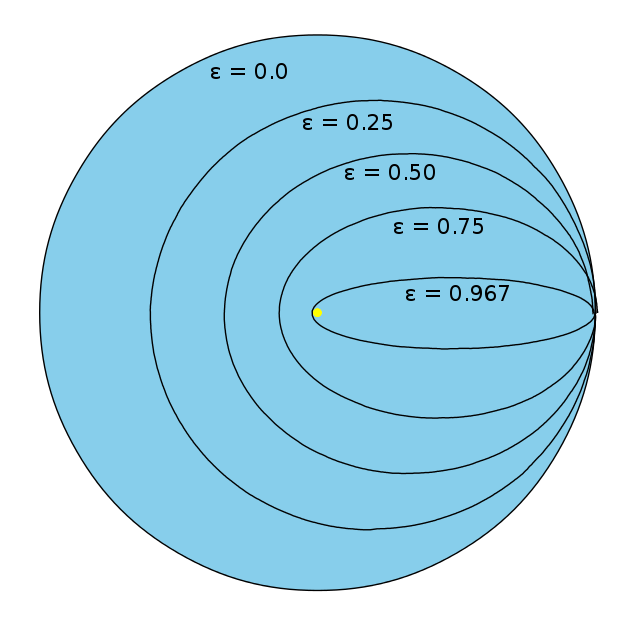
\includegraphics[width=12.0cm]{./images/cerchio/orbite.png}
   \caption{Orbite di un corpo celeste intorno al sole con diversi valori di
	eccentricità $\epsilon$. Il valore $\epsilon$ = 0.967 corrisponde a quello della cometa di Halley..}
   \label{orbite-halley}
\end{figure}

Successivamente vengono determinate le condizioni iniziali, che è un passo fondamentale per la risoluzione di qualsiasi problema di fisica. Se gli allievi uscissero dalle scuole superiori con questo concetto ben  chiaro in testa sarebbe già un gran risultato. L'impostazione computazionale dei problemi di fisica consentirebbe di realizzare questo obiettivo. Nel caso della soluzione di un problema di moto le condizioni iniziali si determinano attraverso la posizione e la velocità iniziali, in valore (modulo) e direzione. Nel nostro codice posizione e dimensioni dell'orbita sono aggiustate in maniera da accomodarsi adeguatamente nella pagina. L'eccentricità invece viene determinata attraverso la II legge di Keplero che lega questa alla velocità del corpo celeste nella sua orbita. In virtù di tale legge, la velocità  di un corpo celeste è legata alla distanza $r$ dal sole mediante questa relazione

\begin{equation} \label{eq:keplero-II}
v = \sqrt{GM(\frac{2}{r}-\frac{1}{a})}
\end{equation}

dove $G$ la costante di gravitazione universale, $M$ è la massa del sole e $a$ è il semiasse maggiore dell'orbita ellittica. Per stabilire la nostra condizione iniziale assumiamo che l'orbita ellittica debba stare sdraiata con l'asse maggiore orizzontale, con il fuoco sinistro coincidente con il centro della pagina e che la cometa "parta" dall'afelio, ovvero nel punto di massima distanza, che così ci ritroviamo a destra, e sia diretta verso il basso. La posizione è determinata mediante le istruzioni 206 e 207. Per quanto riguarda la velocità usiamo il fatto che, quando la distanza dal sole coincide con l'afelio, $r=r_a$, vale la seguente relazione fra la distanza all'afelio $r_a$, il semiasse maggiore $a$ e l'eccentricità $\epsilon$:

\begin{equation}
r_a=a(1+\epsilon) 
\end{equation}

Questa, combinata con l'equazione \ref{eq:keplero-II} fornisce

\begin{equation}
v=\sqrt{\frac{GM}{r_a}(1-\epsilon)}
\end{equation}

che è esattamente l'equazione codificata nell'istruzione 225 del listato, per la componente lungo $y$ della velocità, essendo la componente lungo $x$ pari a 0 perché appunto assumiamo che la cometa in quel punto sia diretta esattamente in basso.

Si comprende qui come, per variare la forma dell'orbita, si possa agire sulla velocità: velocità iniziali maggiori comportano valori di $\epsilon$ inferiori, i quali a loro volta descrivono orbite sempre più circolari. Qui abbiamo dunque la possibilità apprezzare come si possa riflettere sul significato di una formula manipolando il codice software che la esprime, in una maniera che assai difficilmente può verificarsi attraverso la semplice memorizzazione della formula.

Infine, fra l'istruzione 252 e 260 si svolge il ciclo sui punti della traiettoria, dove vengono invocate successivamente le procedure STEP e WRITEPOINT, la prima che calcola il prossimo passo e la seconda che disegna e memorizza i punti calcolati. La variabile yIsNegative, usata come \textit{flag}, ovvero come semaforo sì-no, serve a controllare che l'orbita non venga ripetuta una seconda volta.  Invece la variabile nWrite, usata come contatore, serve a far sì che i punti vengano disegnati e memorizzati sempre ma solo uno ogni tanto, precisamente uno ogni 10000 in questa versione! Ciò è dovuto al fatto che affinché l'orbita venga disegnata con ragionevole precisione, questa venga calcolata con un campionamento molto fitto: in questa implementazione la Tartaruga calcola più di 14 milioni di punti! Non avrebbe senso farle scrivere tutti questi valori e il sistema grafico andrebbe nel pallone perché non possiede questa precisione. Pur tenendo traccia di un punto su diecimila, il numero di punti totale che vengono effettivamente rappresentati e memorizzati è di 1466. Noi ci siamo fermati qui. In realtà sarebbe possibile aggiungere un altro perfezionamento. Ora il campionamento è svolto in modo regolare, con un passo Dt pari a 0.001, che produce oltre 14 milioni di punti, come abbiamo visto. Il risultato ai nostri fini è soddisfacente: l'orbita viene abbastanza regolare e il calcolo si svolge in pochi minuti, anche su un computer moderatamente veloce.  Ma non è detto che non si presentino problemi provando altre configurazioni. In tal caso, potremmo provare a rendere l'interpolazione adattiva, aggiustando il passo Dt in funzione della curvatura della traiettoria: dove questa è più rettilinea la Tartaruga potrebbe procedere spedita, facendo passi più lunghi, mentre dove è più curva i passi potrebbero stringersi progressivamente.

E a proposito di altre configurazioni, lo spazio per le esplorazioni è
sconfinato. Ad esempio, perché non cogliere l'occasione di conoscere Ardusat,
iniziando a simularne l'orbita, anche per farsi un'idea di come "volino" i
satelliti intorno alla terra – una cosa ben diversa dal caso della cometa!
Ardusat\footnote{Informazioni dettagliate si trovano ad esempio
http://www.dk3wn.info/sat/afu/sat\_ardusat.shtml e https://en.wikipedia.org/wiki/ArduSat.} è un cosiddetto "nanosatellite", un cubo di 10 cm di lato che pesa un
chilo – un cartone di latte più o meno – equipaggiato con una particolare
versione di Arduino, basata su 16 microprocessori e uno di controllo più una
serie di 25 sensori diversi, fra cui una videocamera uno spettrometro ottico,
un contatore Geiger, un sensore a infrarossi ecc. È  concepito per essere usato
da studenti, insegnanti o appassionati che possono progettare esperimenti,
applicazioni che impiegano dati spaziali o addirittura giochi. Gli utenti
possono progettare il software delle loro applicazioni sulle normali schede
Arduino per poi sperimentarlo su un clone terrestre di
Ardusat. Quando tutto va bene il software viene inviato a Ardusat per eseguire le operazioni previste, scaricando i dati sul browser degli utenti, quando il satellite è visibile dalle apposite stazioni terrestri. Al termine del periodo di lavoro, che può durare fino a una settimana, tutti dati vengono scaricati e inviati all'utente. In un programma di scienze, potrebbe essere estremamente stimolante esplorare Ardusat, partendo per esempio dalla simulazione della sua orbita con Logo.

Tutte considerazioni che possono essere estremamente istruttive e che possono essere svolte per dare una corretta valutazione di cosa sia oggi la scienza, in particolare di quanto e come gli aspetti computazionali influiscano su di essa. In realtà la riflessione è passibile di un ulteriore e significativo approfondimento, secondo la linea di pensiero illustrata da B. Sherin in un articolo intitolato "\textit{A comparison of programming languages and algebraic notation as expressive languages} for physics"\cite{Sherin}.

Sherin nel suo articolo affianca – si badi bene, non contrappone – la \textit{programming-physics} all'\textit{algebra-physics}. L'impianto teorico del suo lavoro si fonda sul ruolo giocato dalle rappresentazioni strumentali e simboliche che supportano la conoscenza nella formazione stessa di tale conoscenza – concetti sviluppati da altri autori, ad esempio da Weintrop e Wilensky\cite{Weintrop2}. L'autore documenta i propri argomenti con alcuni esercizi di fisica presentati sia nella forma algebrica convenzionale che nella forma computazionale. Per quest'ultima riferisce di esperienze svolte con l'ambiente Boxer, sviluppato da Di Sessa e altri autori\cite{DiSessa}, sulla base di Logo. Con questo lavoro l'autore sostiene la tesi che sistemi di rappresentazione diversi influiscono in modo differente sui meccanismi del pensiero e possono indurre un diverso tipo di comprensione dei medesimi fenomeni. In capo a un'analisi minuziosa di esperimenti didattici, condotti su gruppi di studenti sia mediante l'\textit{algebra-physics} che la \textit{programming-physics}, giunge alla conclusione per cui con la conoscenza algebrica si tende a enfatizzare gli equilibri mentre con quella computazionale si è portati a comprendere meglio gli aspetti dinamici. È estremamente interessante la prospettiva nella quale Sherin pone questa conclusione. Non si tratta, dice, di giudicare l'effetto di un metodo o dell'altro secondo una singola metrica e di confrontarli sulla base di tale metrica – ovvero non si tratta di stabilire quale sia "meglio" - bensì di accettare, comprendere e utilizzare proficuamente il fatto che il nuovo paradigma offra una mutata visione della conoscenza degli stessi fenomeni e di come, in ultima analisi, la cosa più sensata da fare sia quella di affiancare questa nuova forma di conoscenza a quelle preesistenti. E non si può evitare di osservare che la nuova prospettiva computazionale – qui nel senso della \textit{programming-physics} di Sherin, possa essere di grande giovamento per la comprensione dei fenomeni fisici. Infatti lo strumento matematico costituisce indubbiamente il fondamento imprescindibile delle scienze di base – il linguaggio che consente di porre domande alla natura, per dirla con Galileo - ma il processo con il quale un giovane giunge a creare senso compiuto a partire da un linguaggio formale è molto complesso e faticoso. Pochi studenti arrivano ad apprezzare il formalismo matematico come uno strumento utile per comprendere e esprimere pensieri sul mondo fisico o altro. Per la grande maggioranza i formalismi matematici rappresentano al più una quantità di regole da applicare a memoria negli specifici contesti creati dalla scuola: qual era la formula da usare qui...? A questo proposito è interessante ricordare un noto articolo scritto da Enrico Persico\cite{Persico}, maestro di Enrico Fermi, dove ci si domandava cosa non andasse con quella studentessa che procedeva come una locomotiva quando sciorinava le equazioni di Maxwell alla lavagna ma che non sapeva dire perché, con quel certo valore di corrente, una lampadina si sarebbe fulminata – non a caso Sherin rileva esattamente lo stesso problema a pag. 43 del suo lavoro, e proprio a proposito delle equazioni di Maxwell. La questione della comprensione dei fenomeni attraverso il linguaggio matematico non è, e non da ora, semplice. È esattamente qui che il "nuovo" approccio computazionale, nel quale peraltro vengono declinati settori sempre più ampi della fisica e delle altre scienze, può venire in aiuto. Infatti, l'approccio computazionale induce ad analizzare e scomporre i fenomeni fisici nella dimensione temporale, enfatizzandone così la natura dinamica, spesso più accessibile all'intuizione. Non solo, l'analisi computazionale costringe ad utilizzare precisi valori numerici da assegnare ai parametri fisici coinvolti e questa è una pratica che induce più facilmente gli studenti a ricavare un senso da ciò che studiano.

Ora che abbiamo tirato in ballo l'articolo di Sherin vale la pena di specificare che è proprio grazie a questo lavoro che siamo giunti dal "cerchio alla Papert" alle orbite dei corpi celesti. Sì perché all'inizio ci eravamo messi a riprodurre in Logo gli esercizi esemplificati da Sherin, nel modo più semplice possibile. Riportiamo la progressione qui di seguito.

\vskip 1cm

%https://en.wikibooks.org/wiki/LaTeX/Source_Code_Listings
\lstset{literate=
  {á}{{\'a}}1 {é}{{\'e}}1 {í}{{\'i}}1 {ó}{{\'o}}1 {ú}{{\'u}}1
  {Á}{{\'A}}1 {É}{{\'E}}1 {Í}{{\'I}}1 {Ó}{{\'O}}1 {Ú}{{\'U}}1
  {à}{{\`a}}1 {è}{{\`e}}1 {ì}{{\`i}}1 {ò}{{\`o}}1 {ù}{{\`u}}1
  {À}{{\`A}}1 {È}{{\'E}}1 {Ì}{{\`I}}1 {Ò}{{\`O}}1 {Ù}{{\`U}}1
  {ä}{{\"a}}1 {ë}{{\"e}}1 {ï}{{\"i}}1 {ö}{{\"o}}1 {ü}{{\"u}}1
  {Ä}{{\"A}}1 {Ë}{{\"E}}1 {Ï}{{\"I}}1 {Ö}{{\"O}}1 {Ü}{{\"U}}1
  {â}{{\^a}}1 {ê}{{\^e}}1 {î}{{\^i}}1 {ô}{{\^o}}1 {û}{{\^u}}1
  {Â}{{\^A}}1 {Ê}{{\^E}}1 {Î}{{\^I}}1 {Ô}{{\^O}}1 {Û}{{\^U}}1
  {œ}{{\oe}}1 {Œ}{{\OE}}1 {æ}{{\ae}}1 {Æ}{{\AE}}1 {ß}{{\ss}}1
  {ű}{{\H{u}}}1 {Ű}{{\H{U}}}1 {ő}{{\H{o}}}1 {Ő}{{\H{O}}}1
  {ç}{{\c c}}1 {Ç}{{\c C}}1 {ø}{{\o}}1 {å}{{\r a}}1 {Å}{{\r A}}1
  {€}{{\euro}}1 {£}{{\pounds}}1 {«}{{\guillemotleft}}1
  {»}{{\guillemotright}}1 {ñ}{{\~n}}1 {Ñ}{{\~N}}1 {¿}{{?`}}1
}
\lstset{extendedchars=true, basicstyle=\scriptsize} 
\begin{lstlisting}[frame=single]  % Start your code-block

; Caduta di un grave con accelerazione di gravità costante

CLEARSCREEN
HOME

PENUP
FORWARD 350
RIGHT 180
PENDOWN

XPOS = 0.0
VEL = 0.0
ACC = 9.8
DVEL = ACC

REPEAT 10 [
  VEL = VEL + DVEL
  XPOS = XPOS + VEL
  PENDOWN
  CIRCLE 5
  PENUP
  FORWARD VEL
  ]

HIDETURTLE
\end{lstlisting}

\vskip 1cm

%https://en.wikibooks.org/wiki/LaTeX/Source_Code_Listings
\lstset{literate=
  {á}{{\'a}}1 {é}{{\'e}}1 {í}{{\'i}}1 {ó}{{\'o}}1 {ú}{{\'u}}1
  {Á}{{\'A}}1 {É}{{\'E}}1 {Í}{{\'I}}1 {Ó}{{\'O}}1 {Ú}{{\'U}}1
  {à}{{\`a}}1 {è}{{\`e}}1 {ì}{{\`i}}1 {ò}{{\`o}}1 {ù}{{\`u}}1
  {À}{{\`A}}1 {È}{{\'E}}1 {Ì}{{\`I}}1 {Ò}{{\`O}}1 {Ù}{{\`U}}1
  {ä}{{\"a}}1 {ë}{{\"e}}1 {ï}{{\"i}}1 {ö}{{\"o}}1 {ü}{{\"u}}1
  {Ä}{{\"A}}1 {Ë}{{\"E}}1 {Ï}{{\"I}}1 {Ö}{{\"O}}1 {Ü}{{\"U}}1
  {â}{{\^a}}1 {ê}{{\^e}}1 {î}{{\^i}}1 {ô}{{\^o}}1 {û}{{\^u}}1
  {Â}{{\^A}}1 {Ê}{{\^E}}1 {Î}{{\^I}}1 {Ô}{{\^O}}1 {Û}{{\^U}}1
  {œ}{{\oe}}1 {Œ}{{\OE}}1 {æ}{{\ae}}1 {Æ}{{\AE}}1 {ß}{{\ss}}1
  {ű}{{\H{u}}}1 {Ű}{{\H{U}}}1 {ő}{{\H{o}}}1 {Ő}{{\H{O}}}1
  {ç}{{\c c}}1 {Ç}{{\c C}}1 {ø}{{\o}}1 {å}{{\r a}}1 {Å}{{\r A}}1
  {€}{{\euro}}1 {£}{{\pounds}}1 {«}{{\guillemotleft}}1
  {»}{{\guillemotright}}1 {ñ}{{\~n}}1 {Ñ}{{\~N}}1 {¿}{{?`}}1
}
\lstset{extendedchars=true, numbers=left,basicstyle=\scriptsize} 
\begin{lstlisting}[frame=single]  % Start your code-block

; Caduta di un grave con accelerazione di gravità costante
; in presenza di resistenza dell'aria

CLEARSCREEN
HOME

XPOS = 0.0
VEL = 0.0
ACC = 9.8
RES = 0.0

G = 9.8
M = 10.0
K = 2.0

PENUP
FORWARD 350
RIGHT 180
PENDOWN

REPEAT 20 [
  RES = VEL * K
  ACC = G - RES / M
  VEL = VEL + ACC
  XPOS = XPOS + VEL
  PENDOWN
  CIRCLE 5
  PENUP
  FORWARD VEL
  ]

HIDETURTLE
\end{lstlisting}

\vskip 1cm

%https://en.wikibooks.org/wiki/LaTeX/Source_Code_Listings
\lstset{literate=
  {á}{{\'a}}1 {é}{{\'e}}1 {í}{{\'i}}1 {ó}{{\'o}}1 {ú}{{\'u}}1
  {Á}{{\'A}}1 {É}{{\'E}}1 {Í}{{\'I}}1 {Ó}{{\'O}}1 {Ú}{{\'U}}1
  {à}{{\`a}}1 {è}{{\`e}}1 {ì}{{\`i}}1 {ò}{{\`o}}1 {ù}{{\`u}}1
  {À}{{\`A}}1 {È}{{\'E}}1 {Ì}{{\`I}}1 {Ò}{{\`O}}1 {Ù}{{\`U}}1
  {ä}{{\"a}}1 {ë}{{\"e}}1 {ï}{{\"i}}1 {ö}{{\"o}}1 {ü}{{\"u}}1
  {Ä}{{\"A}}1 {Ë}{{\"E}}1 {Ï}{{\"I}}1 {Ö}{{\"O}}1 {Ü}{{\"U}}1
  {â}{{\^a}}1 {ê}{{\^e}}1 {î}{{\^i}}1 {ô}{{\^o}}1 {û}{{\^u}}1
  {Â}{{\^A}}1 {Ê}{{\^E}}1 {Î}{{\^I}}1 {Ô}{{\^O}}1 {Û}{{\^U}}1
  {œ}{{\oe}}1 {Œ}{{\OE}}1 {æ}{{\ae}}1 {Æ}{{\AE}}1 {ß}{{\ss}}1
  {ű}{{\H{u}}}1 {Ű}{{\H{U}}}1 {ő}{{\H{o}}}1 {Ő}{{\H{O}}}1
  {ç}{{\c c}}1 {Ç}{{\c C}}1 {ø}{{\o}}1 {å}{{\r a}}1 {Å}{{\r A}}1
  {€}{{\euro}}1 {£}{{\pounds}}1 {«}{{\guillemotleft}}1
  {»}{{\guillemotright}}1 {ñ}{{\~n}}1 {Ñ}{{\~N}}1 {¿}{{?`}}1
}
\lstset{extendedchars=true, basicstyle=\scriptsize} 
\begin{lstlisting}[frame=single]  % Start your code-block

; Andamento nel tempo del moto di un grave appeso a una molla
; (asse x: tempo)

CLEARSCREEN
HOME

XPOS = 0.0
VEL = 0.0
ACC = 9.8
RES = 0.0

G = 9.8
M = 10.0
KA = 0.5
K = 1.0

PENUP
FORWARD 250
RIGHT 180
PENDOWN

REPEAT [
  RES = KA * VEL
  SPR = K * XPOS
  ACC = G - RES / M - SPR / M 
  VEL = VEL + ACC
  XPOS = XPOS + VEL
  PENDOWN
  CIRCLE 5
  PENUP
  FORWARD VEL
  LEFT 90 FORWARD 3 RIGHT 90 
  ]

HIDETURTLE
\end{lstlisting}

\vskip 1cm

%https://en.wikibooks.org/wiki/LaTeX/Source_Code_Listings
\lstset{literate=
  {á}{{\'a}}1 {é}{{\'e}}1 {í}{{\'i}}1 {ó}{{\'o}}1 {ú}{{\'u}}1
  {Á}{{\'A}}1 {É}{{\'E}}1 {Í}{{\'I}}1 {Ó}{{\'O}}1 {Ú}{{\'U}}1
  {à}{{\`a}}1 {è}{{\`e}}1 {ì}{{\`i}}1 {ò}{{\`o}}1 {ù}{{\`u}}1
  {À}{{\`A}}1 {È}{{\'E}}1 {Ì}{{\`I}}1 {Ò}{{\`O}}1 {Ù}{{\`U}}1
  {ä}{{\"a}}1 {ë}{{\"e}}1 {ï}{{\"i}}1 {ö}{{\"o}}1 {ü}{{\"u}}1
  {Ä}{{\"A}}1 {Ë}{{\"E}}1 {Ï}{{\"I}}1 {Ö}{{\"O}}1 {Ü}{{\"U}}1
  {â}{{\^a}}1 {ê}{{\^e}}1 {î}{{\^i}}1 {ô}{{\^o}}1 {û}{{\^u}}1
  {Â}{{\^A}}1 {Ê}{{\^E}}1 {Î}{{\^I}}1 {Ô}{{\^O}}1 {Û}{{\^U}}1
  {œ}{{\oe}}1 {Œ}{{\OE}}1 {æ}{{\ae}}1 {Æ}{{\AE}}1 {ß}{{\ss}}1
  {ű}{{\H{u}}}1 {Ű}{{\H{U}}}1 {ő}{{\H{o}}}1 {Ő}{{\H{O}}}1
  {ç}{{\c c}}1 {Ç}{{\c C}}1 {ø}{{\o}}1 {å}{{\r a}}1 {Å}{{\r A}}1
  {€}{{\euro}}1 {£}{{\pounds}}1 {«}{{\guillemotleft}}1
  {»}{{\guillemotright}}1 {ñ}{{\~n}}1 {Ñ}{{\~N}}1 {¿}{{?`}}1
}
\lstset{extendedchars=true, basicstyle=\scriptsize} 
\begin{lstlisting}[frame=single]  % Start your code-block

; Caduta di un grave dallo spazio

CLEARSCREEN
HOME

FILLCOLOR "BLUE"
CIRCLE 70
FILLCOLOR "LIME"
XPOS0 = POSITION[0]
YPOS0 = POSITION[1]

PENUP
FORWARD 350
RIGHT 180
PENDOWN
HIDETURTLE

XPOS = POSITION[0]
YPOS = POSITION[1]
VEL = 0.0
KG = 9800

REPEAT [
  DY =  YPOS-YPOS0
  VEL = VEL + KG / DY**2
  YPOS = YPOS + VEL
  PENDOWN
  CIRCLE 5
  IF YPOS0-YPOS < 10 [ BREAK ]
  PENUP
  POSITION [XPOS,YPOS]
;FORWARD (VEL)
  ]
FILLCOLOR "RED"
CIRCLE 10
HEADING 0
FORWARD 5
LABEL "                                               AAAAAAAAH...!!!"                      

HIDETURTLE
\end{lstlisting}

\vskip 1cm
%https://en.wikibooks.org/wiki/LaTeX/Source_Code_Listings
\lstset{literate=
  {á}{{\'a}}1 {é}{{\'e}}1 {í}{{\'i}}1 {ó}{{\'o}}1 {ú}{{\'u}}1
  {Á}{{\'A}}1 {É}{{\'E}}1 {Í}{{\'I}}1 {Ó}{{\'O}}1 {Ú}{{\'U}}1
  {à}{{\`a}}1 {è}{{\`e}}1 {ì}{{\`i}}1 {ò}{{\`o}}1 {ù}{{\`u}}1
  {À}{{\`A}}1 {È}{{\'E}}1 {Ì}{{\`I}}1 {Ò}{{\`O}}1 {Ù}{{\`U}}1
  {ä}{{\"a}}1 {ë}{{\"e}}1 {ï}{{\"i}}1 {ö}{{\"o}}1 {ü}{{\"u}}1
  {Ä}{{\"A}}1 {Ë}{{\"E}}1 {Ï}{{\"I}}1 {Ö}{{\"O}}1 {Ü}{{\"U}}1
  {â}{{\^a}}1 {ê}{{\^e}}1 {î}{{\^i}}1 {ô}{{\^o}}1 {û}{{\^u}}1
  {Â}{{\^A}}1 {Ê}{{\^E}}1 {Î}{{\^I}}1 {Ô}{{\^O}}1 {Û}{{\^U}}1
  {œ}{{\oe}}1 {Œ}{{\OE}}1 {æ}{{\ae}}1 {Æ}{{\AE}}1 {ß}{{\ss}}1
  {ű}{{\H{u}}}1 {Ű}{{\H{U}}}1 {ő}{{\H{o}}}1 {Ő}{{\H{O}}}1
  {ç}{{\c c}}1 {Ç}{{\c C}}1 {ø}{{\o}}1 {å}{{\r a}}1 {Å}{{\r A}}1
  {€}{{\euro}}1 {£}{{\pounds}}1 {«}{{\guillemotleft}}1
  {»}{{\guillemotright}}1 {ñ}{{\~n}}1 {Ñ}{{\~N}}1 {¿}{{?`}}1
}
\lstset{extendedchars=true, basicstyle=\scriptsize} 
\begin{lstlisting}[frame=single]  % Start your code-block

; Legge gravitazionale di Newton in 2D
; È un esempio in germe. Per una corretta e proficua realizzazione 
; didattica occorre entrare nel merito dei valori delle costanti 
; fisiche implicate, masse, distanze, costante gravitazionale, 
; fattori  di scala per la rappresentazione grafica. In questo 
; esempio ho utilizzato valori numerici arbitrari. Interessava 
; vedere come può funzionare... 

; La Tartaruga gioca il ruolo del satellite
; Il pianeta sta al centro, che in LibreLogo ha coordinate 
; [ 297.89, 421.11 ]

CLEARSCREEN
HOME

FILLCOLOR "BLUE"
CIRCLE 20
FILLCOLOR "LIME"
XPOS0 = POSITION[0]
YPOS0 = POSITION[1]
SHOWTURTLE

; Determinazione delle condizioni iniziali

; Posizione iniziale...
; con queste istruzioni la Tartaruga-satellite si dirige nella 
; posizione iniziale lo fa alla Papert, con comandi "sintonici": 
; sale di 100 e poi si mette a testa in giù (fatto inessenziale 
; perché poi la dirigiamo con comandi diretti tramite POSITION)

PENUP
HEADING 9h
FORWARD 0        ; qui si potrebbe spostare lateralmente
HEADING 0
FORWARD 100    ; qui sale di quota
RIGHT 180
PENDOWN

XPOS = POSITION[0]
YPOS = POSITION[1]

; Velocità iniziale...
; dove aggiustando componenti lungo X e Y decidiamo in che 
; direzione lanciare la Tartaruga-satellite (molto divertente 
; giocare con questo...)

; Con XVEL= 10.0 e YVEL=0.0 si azzecca un'orbita circolare
; Con  XVEL= 5.0 e YVEL=0.0 viene l'orbita di tipo caotico mostrata 
; nel post https://iamarf.org/2017/04/19
; /dove-la-tartaruga-di-seymour-papert-impara-la-legge-
; gravitazionale-di-newton/

XVEL = 10.0
YVEL = 0.0

KG = 9800        ; qui dentro ci sarebbero le masse e la costante 
                 ; gravitazionale...

REPEAT 50 [
  DX = (XPOS-XPOS0)
  DY = (YPOS-YPOS0)
  R2 = (DX**2 + DY**2)
  R = SQRT(R2)
  ACC = KG / R2 
  XVEL = XVEL - ACC * DX / R
  YVEL = YVEL - ACC * DY / R
  XPOS = XPOS + XVEL
  YPOS = YPOS + YVEL
  
  PENDOWN
  CIRCLE 5
  IF SQRT((XPOS0-XPOS)**2 + (YPOS0-YPOS)**2) < 10 [ BREAK ]
  PENUP
  POSITION [XPOS, YPOS]
  ]
FILLCOLOR "RED"
CIRCLE 10

HEADING 0
FORWARD 5
LABEL "               AHI!!!"

HIDETURTLE
\end{lstlisting}

\vskip 1cm

Sono codici grezzi, con quasi nessun commento, eccetto l'ultimo, e senza un'accurata identificazione di ciascuna variabile e delle sue unità di misura. Li mettiamo a disposizione affinché possano essere completati e variati dal lettore, un po' come i disegni da colorare per i bambini...

\section{Conclusione}

In questo capitolo la dimensione verticale è ancora più estesa rispetto a quella del capitolo precedente, svolto intorno all'esplorazione di Marta. Qui siamo partiti proprio da un'esperienza che ha avuto luogo in una scuola primaria, dove la maestra Antonella ha coinvolto i suoi bambini in un'esplorazione del cerchio ispirata al pensiero di Papert. Le foto che Antonella ci ha regalato ci hanno come portati in classe. Ci siamo poi serviti delle parole di Papert stesso per commentare come in tale attività fisica si annidi un concetto matematico importante, una "idea potente", quella del calcolo differenziale. Un modo matematico per sviluppare una forma geometrica (in realtà anche molto più di questo) utilizzando solamente "informazioni locali". Ed è proprio Papert che in quel brano collega la questione a quella del calcolo dei movimenti dei corpi celesti, secondo la legge di gravitazione universale di Newton. Nella seconda parte del capitolo ci siamo quindi mossi per esplorare quanto alto possa essere il cielo di Logo, anche in una versione semplificata come quella di LibreLogo. Ed abbiamo preso così sul serio il proposito di andare direttamente nello spazio, provando a calcolare l'orbita di un corpo celeste e scegliendo quella della cometa di Halley, un po' per poterci meravigliare di andare così lontano, seppur nello spazio di un foglio di carta, e un po' per metterci alla prova, perché le orbite delle comete sono molto schiacciate, ovvvero eccentriche, e quindi più insidiose da calcolare. Nel fare tutto ciò abbiamo potuto esplorare aspetti computazionali e di calcolo scientifico niente affatto banali. Anzi, diciamo anche arditi, se li vogliamo pensare calati in una classe di scuola secondaria superiore. Effettivamente, un esercizio del genere non starebbe male nel corso di fisica generale al primo anno di università. Ma questo non significa che non vi possano essere ragazzi più giovani in grado di comprendere un percorso del genere, se adeguatamente seguiti dall'insegnante. Ho conosciuto un ragazzo al IV anno del liceo scientifico, molto vicino a me, al quale davo piccoli incarichi di calcolo scientifico che servivano nel mio lavoro di ricerca. Ebbene, questo ragazzo risolveva questi problemi prima e meglio dei miei giovani collaboratori, assegnisti e dottorandi. La scuola dovrebbe essere in grado di dare sostegno a tutti coloro che esulano dalle medie statistiche, superando il concetto "monodimensionale" e banale di performance, sul raggiungimiento di determinate competenze o altro, ma occupandosi delle diversità e mettendole a frutto. Non è infatti raro che ingegni particolarmente creativi finiscano, in questa scuola ancora largamente tayloristica, fra i "meno bravi".

Infine, abbiamo commentato l'aspetto computazionale dell'esercizio rifacendoci al lavoro di Sherin\cite{Sherin}, autore di un interessante approfondimento sulle differenze fra quella che chiama fisica algebrica, insegnata usualmente, e fisica computazionale. In sostanza, l'approccio computazionale ha il vantaggio di avvicinare maggiormente i ragazzi ai fenomeni, obbligandoli a seguirne gli aspetti dinamici, far capire l'importante concetto di condizione al contorno, che qualsiasi problema di fisica rihciede di affrontare, rendersi maggiormente consapevoli della realtà delle grandezze fisiche in gioco, essendo obbligati a mettervi dei numeri. Abbiamo poi chiuso il capitolo riportando alcuni codici tratti dagli esempi presentati da Sherin nel suo lavoro, in modo che chiunque possa svilupparli e rifinirli, in maniera anloga a quanto abbiamo fatto con il calcolo dell'orbita della cometa di Halley.    

Questo capitolo è anche una risposta ai "detrattori del pensiero computazionale", che duellano nei social network con gli altrettanto sgradevoli entusiasti del "codice facile". Le polemiche che si sviluppano in questi contesti si centrano sovente su una visione automatizzata delle pratiche di coding, come se queste si riducessero a banali sequenze di comandi, inducendo gli allievi all'esecuzione passiva di procedure automatizzate. Ora, io non sono in grado di affermare che le pratiche di coding possano essere applicate con risultati significativi anche in contesti umanistici - penso di sì ma non ho gli elementi per fare affermazioni certe - ma sicuramente, per qualsiasi giovane che sia interessato all'ambito delle discipline STEM, oggi il coding è uno strumento fondamentale. E lo è non solo dal punto di vista strumentale ma profondamente culturale, perché non vi è dominio scientifico che, da più di mezzo secolo a questa parte, non si sia ampiamente esteso grazie alla prospettiva computazionale. Nascondere questo agli studenti che andranno a iscriversi ai corsi di laurea scientifici è una grave omissione da parte della scuola. 
